% Generated by Sphinx.
\def\sphinxdocclass{report}
\documentclass[A4paper,10pt,english]{sphinxmanual}
\usepackage[utf8]{inputenc}
\DeclareUnicodeCharacter{00A0}{\nobreakspace}
\usepackage[T1]{fontenc}
\usepackage{babel}
\usepackage{times}
\usepackage[Bjarne]{fncychap}
\usepackage{longtable}
\usepackage{sphinx}
\usepackage{multirow}


\title{CSjark Documentation}
\date{November 21, 2011}
\release{0.4.2}
\author{Erik Bergersen \and Jaroslav Fibichr \and Sondre Johan Mannsverk \and Terje Snarby \and Even Wiik Thomassen \and Lars Solvoll Tønder \and Sigurd Wien}
\newcommand{\sphinxlogo}{}
\renewcommand{\releasename}{Release}
\makeindex

\makeatletter
\def\PYG@reset{\let\PYG@it=\relax \let\PYG@bf=\relax%
    \let\PYG@ul=\relax \let\PYG@tc=\relax%
    \let\PYG@bc=\relax \let\PYG@ff=\relax}
\def\PYG@tok#1{\csname PYG@tok@#1\endcsname}
\def\PYG@toks#1+{\ifx\relax#1\empty\else%
    \PYG@tok{#1}\expandafter\PYG@toks\fi}
\def\PYG@do#1{\PYG@bc{\PYG@tc{\PYG@ul{%
    \PYG@it{\PYG@bf{\PYG@ff{#1}}}}}}}
\def\PYG#1#2{\PYG@reset\PYG@toks#1+\relax+\PYG@do{#2}}

\def\PYG@tok@gd{\def\PYG@tc##1{\textcolor[rgb]{0.63,0.00,0.00}{##1}}}
\def\PYG@tok@gu{\let\PYG@bf=\textbf\def\PYG@tc##1{\textcolor[rgb]{0.50,0.00,0.50}{##1}}}
\def\PYG@tok@gt{\def\PYG@tc##1{\textcolor[rgb]{0.00,0.25,0.82}{##1}}}
\def\PYG@tok@gs{\let\PYG@bf=\textbf}
\def\PYG@tok@gr{\def\PYG@tc##1{\textcolor[rgb]{1.00,0.00,0.00}{##1}}}
\def\PYG@tok@cm{\let\PYG@it=\textit\def\PYG@tc##1{\textcolor[rgb]{0.25,0.50,0.56}{##1}}}
\def\PYG@tok@vg{\def\PYG@tc##1{\textcolor[rgb]{0.73,0.38,0.84}{##1}}}
\def\PYG@tok@m{\def\PYG@tc##1{\textcolor[rgb]{0.13,0.50,0.31}{##1}}}
\def\PYG@tok@mh{\def\PYG@tc##1{\textcolor[rgb]{0.13,0.50,0.31}{##1}}}
\def\PYG@tok@cs{\def\PYG@tc##1{\textcolor[rgb]{0.25,0.50,0.56}{##1}}\def\PYG@bc##1{\colorbox[rgb]{1.00,0.94,0.94}{##1}}}
\def\PYG@tok@ge{\let\PYG@it=\textit}
\def\PYG@tok@vc{\def\PYG@tc##1{\textcolor[rgb]{0.73,0.38,0.84}{##1}}}
\def\PYG@tok@il{\def\PYG@tc##1{\textcolor[rgb]{0.13,0.50,0.31}{##1}}}
\def\PYG@tok@go{\def\PYG@tc##1{\textcolor[rgb]{0.19,0.19,0.19}{##1}}}
\def\PYG@tok@cp{\def\PYG@tc##1{\textcolor[rgb]{0.00,0.44,0.13}{##1}}}
\def\PYG@tok@gi{\def\PYG@tc##1{\textcolor[rgb]{0.00,0.63,0.00}{##1}}}
\def\PYG@tok@gh{\let\PYG@bf=\textbf\def\PYG@tc##1{\textcolor[rgb]{0.00,0.00,0.50}{##1}}}
\def\PYG@tok@ni{\let\PYG@bf=\textbf\def\PYG@tc##1{\textcolor[rgb]{0.84,0.33,0.22}{##1}}}
\def\PYG@tok@nl{\let\PYG@bf=\textbf\def\PYG@tc##1{\textcolor[rgb]{0.00,0.13,0.44}{##1}}}
\def\PYG@tok@nn{\let\PYG@bf=\textbf\def\PYG@tc##1{\textcolor[rgb]{0.05,0.52,0.71}{##1}}}
\def\PYG@tok@no{\def\PYG@tc##1{\textcolor[rgb]{0.38,0.68,0.84}{##1}}}
\def\PYG@tok@na{\def\PYG@tc##1{\textcolor[rgb]{0.25,0.44,0.63}{##1}}}
\def\PYG@tok@nb{\def\PYG@tc##1{\textcolor[rgb]{0.00,0.44,0.13}{##1}}}
\def\PYG@tok@nc{\let\PYG@bf=\textbf\def\PYG@tc##1{\textcolor[rgb]{0.05,0.52,0.71}{##1}}}
\def\PYG@tok@nd{\let\PYG@bf=\textbf\def\PYG@tc##1{\textcolor[rgb]{0.33,0.33,0.33}{##1}}}
\def\PYG@tok@ne{\def\PYG@tc##1{\textcolor[rgb]{0.00,0.44,0.13}{##1}}}
\def\PYG@tok@nf{\def\PYG@tc##1{\textcolor[rgb]{0.02,0.16,0.49}{##1}}}
\def\PYG@tok@si{\let\PYG@it=\textit\def\PYG@tc##1{\textcolor[rgb]{0.44,0.63,0.82}{##1}}}
\def\PYG@tok@s2{\def\PYG@tc##1{\textcolor[rgb]{0.25,0.44,0.63}{##1}}}
\def\PYG@tok@vi{\def\PYG@tc##1{\textcolor[rgb]{0.73,0.38,0.84}{##1}}}
\def\PYG@tok@nt{\let\PYG@bf=\textbf\def\PYG@tc##1{\textcolor[rgb]{0.02,0.16,0.45}{##1}}}
\def\PYG@tok@nv{\def\PYG@tc##1{\textcolor[rgb]{0.73,0.38,0.84}{##1}}}
\def\PYG@tok@s1{\def\PYG@tc##1{\textcolor[rgb]{0.25,0.44,0.63}{##1}}}
\def\PYG@tok@gp{\let\PYG@bf=\textbf\def\PYG@tc##1{\textcolor[rgb]{0.78,0.36,0.04}{##1}}}
\def\PYG@tok@sh{\def\PYG@tc##1{\textcolor[rgb]{0.25,0.44,0.63}{##1}}}
\def\PYG@tok@ow{\let\PYG@bf=\textbf\def\PYG@tc##1{\textcolor[rgb]{0.00,0.44,0.13}{##1}}}
\def\PYG@tok@sx{\def\PYG@tc##1{\textcolor[rgb]{0.78,0.36,0.04}{##1}}}
\def\PYG@tok@bp{\def\PYG@tc##1{\textcolor[rgb]{0.00,0.44,0.13}{##1}}}
\def\PYG@tok@c1{\let\PYG@it=\textit\def\PYG@tc##1{\textcolor[rgb]{0.25,0.50,0.56}{##1}}}
\def\PYG@tok@kc{\let\PYG@bf=\textbf\def\PYG@tc##1{\textcolor[rgb]{0.00,0.44,0.13}{##1}}}
\def\PYG@tok@c{\let\PYG@it=\textit\def\PYG@tc##1{\textcolor[rgb]{0.25,0.50,0.56}{##1}}}
\def\PYG@tok@mf{\def\PYG@tc##1{\textcolor[rgb]{0.13,0.50,0.31}{##1}}}
\def\PYG@tok@err{\def\PYG@bc##1{\fcolorbox[rgb]{1.00,0.00,0.00}{1,1,1}{##1}}}
\def\PYG@tok@kd{\let\PYG@bf=\textbf\def\PYG@tc##1{\textcolor[rgb]{0.00,0.44,0.13}{##1}}}
\def\PYG@tok@ss{\def\PYG@tc##1{\textcolor[rgb]{0.32,0.47,0.09}{##1}}}
\def\PYG@tok@sr{\def\PYG@tc##1{\textcolor[rgb]{0.14,0.33,0.53}{##1}}}
\def\PYG@tok@mo{\def\PYG@tc##1{\textcolor[rgb]{0.13,0.50,0.31}{##1}}}
\def\PYG@tok@mi{\def\PYG@tc##1{\textcolor[rgb]{0.13,0.50,0.31}{##1}}}
\def\PYG@tok@kn{\let\PYG@bf=\textbf\def\PYG@tc##1{\textcolor[rgb]{0.00,0.44,0.13}{##1}}}
\def\PYG@tok@o{\def\PYG@tc##1{\textcolor[rgb]{0.40,0.40,0.40}{##1}}}
\def\PYG@tok@kr{\let\PYG@bf=\textbf\def\PYG@tc##1{\textcolor[rgb]{0.00,0.44,0.13}{##1}}}
\def\PYG@tok@s{\def\PYG@tc##1{\textcolor[rgb]{0.25,0.44,0.63}{##1}}}
\def\PYG@tok@kp{\def\PYG@tc##1{\textcolor[rgb]{0.00,0.44,0.13}{##1}}}
\def\PYG@tok@w{\def\PYG@tc##1{\textcolor[rgb]{0.73,0.73,0.73}{##1}}}
\def\PYG@tok@kt{\def\PYG@tc##1{\textcolor[rgb]{0.56,0.13,0.00}{##1}}}
\def\PYG@tok@sc{\def\PYG@tc##1{\textcolor[rgb]{0.25,0.44,0.63}{##1}}}
\def\PYG@tok@sb{\def\PYG@tc##1{\textcolor[rgb]{0.25,0.44,0.63}{##1}}}
\def\PYG@tok@k{\let\PYG@bf=\textbf\def\PYG@tc##1{\textcolor[rgb]{0.00,0.44,0.13}{##1}}}
\def\PYG@tok@se{\let\PYG@bf=\textbf\def\PYG@tc##1{\textcolor[rgb]{0.25,0.44,0.63}{##1}}}
\def\PYG@tok@sd{\let\PYG@it=\textit\def\PYG@tc##1{\textcolor[rgb]{0.25,0.44,0.63}{##1}}}

\def\PYGZbs{\char`\\}
\def\PYGZus{\char`\_}
\def\PYGZob{\char`\{}
\def\PYGZcb{\char`\}}
\def\PYGZca{\char`\^}
\def\PYGZsh{\char`\#}
\def\PYGZpc{\char`\%}
\def\PYGZdl{\char`\$}
\def\PYGZti{\char`\~}
% for compatibility with earlier versions
\def\PYGZat{@}
\def\PYGZlb{[}
\def\PYGZrb{]}
\makeatother

\begin{document}

% \maketitle
% \tableofcontents
% \phantomsection\label{index::doc}


CSjark is a tool for generating Lua dissectors from C struct definitions to use with Wireshark. \href{http://www.wireshark.org}{Wireshark} is a leading tool for capturing and analysing network traffic. CSjark provides a way to display the contents of the C struct data coming from an IPC packet in human-readable form in Wireshark.

You can find more about CSjark functionality in the {\hyperref[user/intro:intro]{\emph{Introduction}}} section.


\chapter{User Documentation}
\label{index:user-documentation}\label{index:welcome-to-csjark-s-documentation}

\section{Introduction}
\label{user/intro:introduction}\label{user/intro:intro}\label{user/intro::doc}
This part is a technical introduction to CSjark. It gives a concise explanation of the most important terms used in the documentation.
The first section briefly explains Wireshark, dissectors and how dissectors are used in Wireshark. The connection between Wireshark and the Lua structs protocol is also explained. The second section describes how the Lua code works and how it is generated by our utility.


\subsection{Wireshark and dissectors}
\label{user/intro:wireshark-and-dissectors}
This section gives a brief introduction to Wireshark and dissectors. The
rst part describes what Wireshark is and what it can be used for. The second part explains exactly what a dissector is, and how a dissector can be used to extend Wireshark.


\subsubsection{Wireshark}
\label{user/intro:wireshark}
\href{http://www.wireshark.org}{Wireshark} is a program used to analyze network traffic. A common usage scenario is when a person wants to troubleshoot network problems or look at the internal workings of a network protocol. An important feature of Wireshark is the ability to capture and display a live stream of packets sent through the network. A user could, for example, see exactly what happens when he opens up a website. Wireshark will then display all the messages sent between his computer and the web server. It is also possible to filter and search on given packet attributes, which facilitates the debugging process.

In {\hyperref[user/intro:figure-1]{Figure 1}}, you can see a view of Wireshark. This specific example shows a capture file with four messages, or packets, sent between internal 2 processes, in other words it is a view of messages sent by inter-process communication. Each of the packets contain one C struct. To be able to display the contents of the C struct, Wireshark has to be extended. This can be accomplished by writing a dissector for the C struct.
\begin{figure}[htbp]
\centering
\capstart

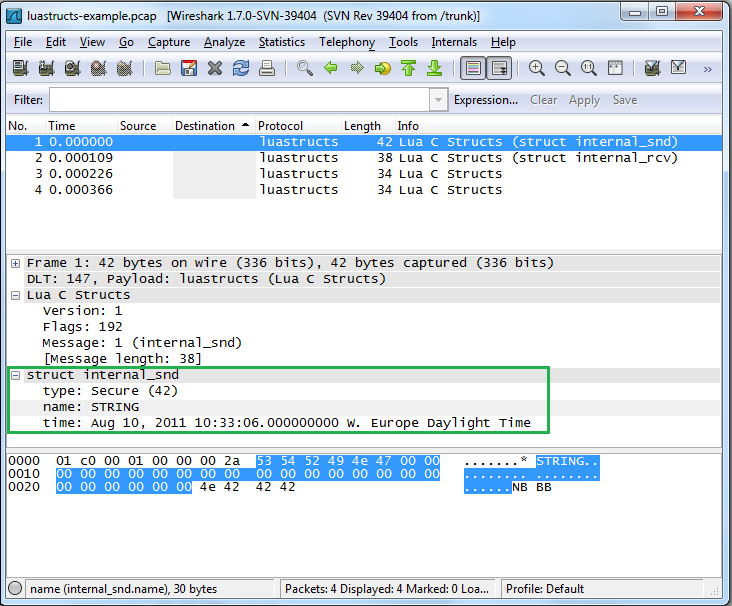
\includegraphics[width=\linewidth]{img/wireshark_example.png}
\caption{\emph{Figure 1:} Wireshark}\label{user/intro:figure-1}\end{figure}


\subsubsection{Dissector}
\label{user/intro:dissector}
In short, a dissector is a piece of code, run on a blob of data, which can dissect the data and display it in a readable format in Wireshark, instead of the binary representation.
The {\hyperref[user/intro:figure-1]{Figure 1}} displays four packets, with packet number 1 highlighted. The content of the packet is a C struct with two members, name and time, and it is displayed inside the green box. The C code for the struct is shown below.

\begin{Verbatim}[commandchars=\\\{\}]
/*
* Sample header file for testing Lua C structs script
* Copyright 2011 , Stig Bjorlykke \textless{}stig@bjorlykke.org\textgreater{}
*/

\#include \textless{}time.h\textgreater{}

\#define STRING\_LEN 30

struct internal\_snd \PYGZob{}
    int type;
    char name [STRING\_LEN];
    time\_t time;
\PYGZcb{};
\end{Verbatim}

The dissector takes the C struct, decodes its binary representation and makes it readable by humans. Without a dissector, Wireshark would just display the struct and struct members as a binary blob.

All the packets containing C structs belong to the protocol called \code{luastructs}. When opening a capture file in Wireshark, this protocol maps the id of the messages to the correct dissector, and calls them.


\subsection{From struct definition to Lua dissector}
\label{user/intro:from-struct-definition-to-lua-dissector}
This section explains what happens under the hood of a Lua dissector.


\subsubsection{Lua dissectors}
\label{user/intro:lua-dissectors}
The code below shows what the code for the Lua dissector, displayed in packet 1 in {\hyperref[user/intro:figure-1]{Figure 1}}, looks like. The \code{Proto} variable defines a new protocol. In this example, a dissector for the internal\_snd struct, called internal\_snd, is created. The different fields of the struct are created as instances of \code{ProtoField}, and put in \code{Protocol.fields}. For example, the \code{name} variable is a string in C, and as such it is created as a ProtoField.string with the name \code{name}.

The protocol dissector method is the method that does the actual dissecting. A subtree for the dissector is created, and the description of the dissector is appended to the information column. All the ProtoFields are added to the subtree. Here you can see that the \code{type}, \code{name} and \code{time} fields are added to the subtree for the \code{internal\_snd} dissector. The buffer size allocated to the fields is the size of the members in C.

\begin{Verbatim}[commandchars=\\\{\}]
--
--  A sample dissector for testing Lua C structs scripts
--  Copyright 2011, Stig Bjorlykke \textless{}stig@bjorlykke.org\textgreater{}
--

local PROTOCOL = Proto ("internal\_snd", "struct internal\_snd")
local luastructs\_dt = DissectorTable.get ("luastructs.message")

local types = \PYGZob{} [0] = "None", [1] = "Regular", [42] = "Secure" \PYGZcb{}

local f = PROTOCOL.fields
f.type = ProtoField.uint32 ("internal\_snd.type", "type", nil, types)
f.time = ProtoField.absolute\_time ("internal\_snd.time", "time")
f.name = ProtoField.string ("internal\_snd.name", "name")

function PROTOCOL.dissector (buffer, pinfo, tree)
   local subtree = tree:add (PROTOCOL, buffer())
   pinfo.cols.info:append (" (" .. PROTOCOL.description .. ")")

   subtree:add (f.type, buffer(0,4))
   subtree:add (f.name, buffer(4,30))
   subtree:add (f.time, buffer(34,4))
end

luastructs\_dt:add (1, PROTOCOL)
\end{Verbatim}

\begin{description}
\item[Note]
% \begin{notice}{note}{Note:}
Lua dissectors are usually files with extension \code{.lua}.
% \end{notice}
\end{description}

For further information on the Lua integration in Wireshark, please visit:
\href{http://www.wireshark.org/docs/wsug\_html\_chunked/wsluarm.html}{Lua Support in Wireshark}.

More information programming in Lua in general can be found in \href{http://www.lua.org/manual/5.1/}{Lua reference manual}.


\section{Features}
\label{user/features::doc}\label{user/features:features}
This is a list of CSjark features:
\begin{itemize}
\item {} 
C header files

\item {} 
Batch mode

\item {} 
Searching and filtering in Wireshark

\item {} 
...

\end{itemize}


\subsection{Currently supported platforms}
\label{user/features:currently-supported-platforms}\begin{itemize}
\item {} 
Windows 32-bit

\item {} 
Windows 64-bit

\item {} 
Solaris 32-bit

\item {} 
Solaris 64-bit

\item {} 
Solaris SPARC 64-bit

\item {} 
MacOS

\item {} 
Linux 32 bit

\end{itemize}

(additional platforms can be added by configuration)


\section{Installing CSjark}
\label{user/install::doc}\label{user/install:installing-csjark}

\subsection{Dependencies}
\label{user/install:dependencies}
CSjark is written in Python 3.2, and therefore needs Python 3.2 (or later) to run. Latest implementation of Python can be downloaded from \href{http://www.python.org/}{Python website}. For installing please follow the instruction found there.

There are 4 third party dependencies to get CSjark working:
\begin{enumerate}
\item {} \begin{description}
\item[{\textbf{PLY} (Python Lex-Yacc)}] \leavevmode
PLY is an implementation of lex and yacc parsing tools for Python. It is required by pycparser. Instructions and further information can be found on the page linked above.

\begin{tabulary}{\linewidth}{|L|L|}
\hline

\textbf{Required version}
 & 
3.4
\\\hline

\textbf{Download location}
 & 
\href{http://www.dabeaz.com/ply/}{http://www.dabeaz.com/ply/}
\\\hline
\end{tabulary}


\end{description}

\item {} \begin{description}
\item[{\textbf{pycpaser}}] \leavevmode
\href{http://code.google.com/p/pycparser/}{Pycparser} is a C parser (and AST generator) implemented in Python. Due to the continuous development, CSjark requires the latest development version (not the release version).

\begin{tabulary}{\linewidth}{|L|L|}
\hline

\textbf{Required version}
 & 
latest development version from pycparser repository
\\\hline

\textbf{Download location}
 & 
pycparser repository: \href{http://code.google.com/p/pycparser/source/checkout}{http://code.google.com/p/pycparser/source/checkout}
\\\hline
\end{tabulary}


\end{description}

\item {} \begin{description}
\item[{\textbf{C  preprocessor}}] \leavevmode
CSjark requires a C-preprocessor. The way how to get one depends on operating system used by the user:

\begin{tabulary}{\linewidth}{|L|L|}
\hline

\textbf{Windows}
 & 
Bundled with CSjark.
\\\hline

\textbf{OS X, Linux, Solaris}
 & 
Needs to be installed separately. For example, as a part of \href{http://gcc.gnu.org/}{GCC}
\\\hline
\end{tabulary}


\end{description}

\item {} 
\textbf{pyYAML}
\begin{quote}

\href{http://pyyaml.org/wiki/PyYAML}{pyYAML} is a YAML parser and emitter for the Python programming language. \href{http://yaml.org/}{YAML} is a standard used to specify configurations to CSjark. The website includes both a way to download the software and also instructions of how to install it.

\begin{tabulary}{\linewidth}{|L|L|}
\hline

\textbf{Required version}
 & 
3.10
\\\hline

\textbf{Download location}
 & 
\href{http://pyyaml.org/wiki/PyYAML}{http://pyyaml.org/wiki/PyYAML}
\\\hline
\end{tabulary}

\end{quote}

\end{enumerate}


\subsection{Wireshark}
\label{user/install:ws}\label{user/install:wireshark}
\href{http://www.wireshark.org/}{Wireshark} is an open source protocol analyzer which can use the Lua dissectors generated by CSjark. To get the proper integration of Lua dissectors, the latest development version of Wireshark is required.

\begin{tabulary}{\linewidth}{|L|L|}
\hline

\textbf{Required version}
 & 
1.7 dev (build 39446 or newer)
\\\hline

\textbf{Download location}
 & 
\href{http://www.wireshark.org/download/automated/}{http://www.wireshark.org/download/automated/}, on the page, browse for the required platform version
\\\hline
\end{tabulary}



\subsection{CSjark}
\label{user/install:csjark}
CSjark can be obtained at git CSjark repository: \href{https://github.com/eventh/kpro9/}{https://github.com/eventh/kpro9/}.
CSjark itself requires no installation. After the steps described in the dependencies section is completed. It can be ran by opening a terminal, navigating to the directory containing \code{cshark.py} and invoking as described in section {\hyperref[user/use:use]{\emph{Using CSjark}}}.


\section{Using CSjark}
\label{user/use:using-csjark}\label{user/use:use}\label{user/use::doc}
CSjark can be invoked by running the \code{csjark.py} script. The arguments must be specified according to:

\begin{Verbatim}[commandchars=\\\{\}]
csjark.py [-h] [-v] [-d] [-s] [-f [header [header ...]]]
          [-c [config [config ...]]] [-x [path [path ...]]]
          [-o [output]] [-p] [-n] [-C [path]] [-i [header [header ...]]]
          [-I [directory [directory ...]]]
          [-D [name=definition [name=definition ...]]]
          [-U [name [name ...]]] [-A [argument [argument ...]]]
          [header] [config]
\end{Verbatim}

\textbf{Example usage:}

\begin{Verbatim}[commandchars=\\\{\}]
python csjark.py -v -o dissectors headerfile.h configfile.yml
\end{Verbatim}

\textbf{Batch mode}

One of the most important features of CSjark is processing multiple C header files in one run. That can be easily achieved by specifying a directory instead of a single file as command line argument (see above):

\begin{Verbatim}[commandchars=\\\{\}]
python csjark.py headers configs
\end{Verbatim}

In batch mode, CSjark only generates dissectors for structs that have a configuration file with an ID (see section {\hyperref[user/config:ids]{\emph{Dissector message ID}}} for information how to specify dissector message ID), and for structs that depend on other structs. This speeds up the generation of dissectors, since it only generates dissectors that Wireshark can use.

\textbf{Required arguments}
\begin{description}
\item[{\code{header}}] \leavevmode
a C header file to parse or directory which includes header files

\item[{\code{config}}] \leavevmode
a configuration file to parse or directory which includes configuration files

\end{description}

Both \code{header} and \code{config} can be:
\begin{itemize}
\item {} 
file - CSjark processes only the specified file

\item {} 
directory - CSjark recursively searches the directory and processes all the appropriate files found

\end{itemize}

\textbf{Optional argument list}

\begin{tabulary}{\linewidth}{|L|L|}
\hline

{\hyperref[user/use:cmdoption-h]{\emph{\texttt{-h}}}}, {\hyperref[user/use:cmdoption-h]{\emph{\texttt{-{-}help}}}}
 & 
Show a help message and exit.
\\\hline

{\hyperref[user/use:cmdoption-v]{\emph{\texttt{-v}}}}, {\hyperref[user/use:cmdoption-v]{\emph{\texttt{-{-}verbose}}}}
 & 
Print detailed information.
\\\hline

{\hyperref[user/use:cmdoption-d]{\emph{\texttt{-d}}}}, {\hyperref[user/use:cmdoption-d]{\emph{\texttt{-{-}debug}}}}
 & 
Print debugging information.
\\\hline

{\hyperref[user/use:cmdoption-s]{\emph{\texttt{-s}}}}, {\hyperref[user/use:cmdoption-s]{\emph{\texttt{-{-}strict}}}}
 & 
Only generate dissectors for known structs.
\\\hline

{\hyperref[user/use:cmdoption-f]{\emph{\texttt{-f}}}}, {\hyperref[user/use:cmdoption-f]{\emph{\texttt{-{-}file}}}}
 & 
Additional locations of header files.
\\\hline

{\hyperref[user/use:cmdoption-c]{\emph{\texttt{-c}}}}, {\hyperref[user/use:cmdoption-c]{\emph{\texttt{-{-}config}}}}
 & 
Additional locations of configuration files.
\\\hline

{\hyperref[user/use:cmdoption-x]{\emph{\texttt{-x}}}}, {\hyperref[user/use:cmdoption-x]{\emph{\texttt{-{-}exclude}}}}
 & 
File or folders to exclude from parsing.
\\\hline

{\hyperref[user/use:cmdoption-o]{\emph{\texttt{-o}}}}, {\hyperref[user/use:cmdoption-o]{\emph{\texttt{-{-}output}}}}
 & 
Location for storing generated dissectors.
\\\hline

{\hyperref[user/use:cmdoption-p]{\emph{\texttt{-p}}}}, {\hyperref[user/use:cmdoption-p]{\emph{\texttt{-{-}placeholders}}}}
 & 
Automatically generates config files with placeholders.
\\\hline

{\hyperref[user/use:cmdoption-n]{\emph{\texttt{-n}}}}, {\hyperref[user/use:cmdoption-n]{\emph{\texttt{-{-}nocpp}}}}
 & 
Disables the C pre-processor.
\\\hline

{\hyperref[user/use:cmdoption-C]{\emph{\texttt{-C}}}}, {\hyperref[user/use:cmdoption-C]{\emph{\texttt{-{-}Cpppath}}}}
 & 
Specifies the path to C preprocessor.
\\\hline

{\hyperref[user/use:cmdoption-i]{\emph{\texttt{-i}}}}, {\hyperref[user/use:cmdoption-i]{\emph{\texttt{-{-}include}}}}
 & 
Process file as Cpp \emph{\#include ``file''} directive
\\\hline

{\hyperref[user/use:cmdoption-I]{\emph{\texttt{-I}}}}, {\hyperref[user/use:cmdoption-I]{\emph{\texttt{-{-}Includes}}}}
 & 
Additional directories to be searched for Cpp includes.
\\\hline

{\hyperref[user/use:cmdoption-D]{\emph{\texttt{-D}}}}, {\hyperref[user/use:cmdoption-D]{\emph{\texttt{-{-}Define}}}}
 & 
Predefine name as a Cpp macro
\\\hline

{\hyperref[user/use:cmdoption-U]{\emph{\texttt{-U}}}}, {\hyperref[user/use:cmdoption-U]{\emph{\texttt{-{-}Undefine}}}}
 & 
Cancel any previous Cpp definition of name
\\\hline

{\hyperref[user/use:cmdoption-A]{\emph{\texttt{-A}}}}, {\hyperref[user/use:cmdoption-A]{\emph{\texttt{-{-}Additional}}}}
 & 
Any additional C preprocessor arguments
\\\hline
\end{tabulary}


\textbf{Optional argument details}
\index{command line option!-h, --help}\index{-h, --help!command line option}

\begin{fulllineitems}
\phantomsection\label{user/use:cmdoption-h}\pysigline{\bfcode{-h}\code{}\code{,~}\bfcode{--help}\code{}}
Show a help message and exit.

\end{fulllineitems}

\index{command line option!-v, --verbose}\index{-v, --verbose!command line option}

\begin{fulllineitems}
\phantomsection\label{user/use:cmdoption-v}\pysigline{\bfcode{-v}\code{}\code{,~}\bfcode{--verbose}\code{}}
Print detailed information.

\end{fulllineitems}

\index{command line option!-d, --debug}\index{-d, --debug!command line option}

\begin{fulllineitems}
\phantomsection\label{user/use:cmdoption-d}\pysigline{\bfcode{-d}\code{}\code{,~}\bfcode{--debug}\code{}}
Print debugging information.

\end{fulllineitems}

\index{command line option!-s, --strict}\index{-s, --strict!command line option}

\begin{fulllineitems}
\phantomsection\label{user/use:cmdoption-s}\pysigline{\bfcode{-s}\code{}\code{,~}\bfcode{--strict}\code{}}
Only generate dissectors for known structs. As known structs we consider only structs for which exists valid configuration file with ID defined. Also, CSjark generates dissectors for structs that depend on known structs.

\end{fulllineitems}

\index{command line option!-f {[}path {[}path ...{]}{]}, --file {[}path {[}path ...{]}{]}}\index{-f {[}path {[}path ...{]}{]}, --file {[}path {[}path ...{]}{]}!command line option}

\begin{fulllineitems}
\phantomsection\label{user/use:cmdoption-f}\pysigline{\bfcode{-f}\code{~{[}path~{[}path~...{]}{]}}\code{,~}\bfcode{--file}\code{~{[}path~{[}path~...{]}{]}}}
Specifies that CSjark looks for struct definitions in the \emph{path}. There can be more than one path specified, separated by whitespace. As \emph{path} there can be file and directory. In case of a directory, CSjark searches for header files recursively to maximum possible depth.

All header files found are added to the files specified by the required \code{header} argument.

Example:

\begin{Verbatim}[commandchars=\\\{\}]
csjark.py -f hdr/file1.h dir1 file2.h
\end{Verbatim}

\end{fulllineitems}

\index{command line option!-c {[}path {[}path ...{]}{]}, --config {[}path {[}path ...{]}{]}}\index{-c {[}path {[}path ...{]}{]}, --config {[}path {[}path ...{]}{]}!command line option}

\begin{fulllineitems}
\phantomsection\label{user/use:cmdoption-c}\pysigline{\bfcode{-c}\code{~{[}path~{[}path~...{]}{]}}\code{,~}\bfcode{--config}\code{~{[}path~{[}path~...{]}{]}}}
Specifies that CSjark looks for configuration definition files in the \emph{path}. There can be more than one path specified, separated by whitespace. As \emph{path} there can be file and directory. In case of a directory, CSjark searches for configuration files recursively to maximum possible depth.

All configuration files found are added to the files specified by the required \code{config} argument.

Example:

\begin{Verbatim}[commandchars=\\\{\}]
csjark.py -c etc/conf1.yml dir1 conf2.yml
\end{Verbatim}

\end{fulllineitems}

\index{command line option!-x {[}path {[}path ...{]}{]}, --exclude {[}path {[}path ...{]}{]}}\index{-x {[}path {[}path ...{]}{]}, --exclude {[}path {[}path ...{]}{]}!command line option}

\begin{fulllineitems}
\phantomsection\label{user/use:cmdoption-x}\pysigline{\bfcode{-x}\code{~{[}path~{[}path~...{]}{]}}\code{,~}\bfcode{--exclude}\code{~{[}path~{[}path~...{]}{]}}}
File or folders to exclude from parsing.

When using the option, CSjark will not search for header files in the \emph{path}. There can be more than one path specified, separated by whitespace. As \emph{path} there can be file and directory. In case of a directory, CSjark will skip header files also in its subdirectories.

\end{fulllineitems}

\index{command line option!-o {[}path{]}, --output {[}path{]}}\index{-o {[}path{]}, --output {[}path{]}!command line option}

\begin{fulllineitems}
\phantomsection\label{user/use:cmdoption-o}\pysigline{\bfcode{-o}\code{~{[}path{]}}\code{,~}\bfcode{--output}\code{~{[}path{]}}}
Sets location for storing generated dissectors.

If \emph{path} is a directory, CSjark saves the output dissectors into this directory, otherwise CSjark saves the output dissectors into one specified file named \emph{path}. If file with this name already exists, it is rewritten without warning.

\emph{Default:} CSjark root directory (when the \emph{csjark.py} file is located)

\end{fulllineitems}

\index{command line option!-p, --placeholders}\index{-p, --placeholders!command line option}

\begin{fulllineitems}
\phantomsection\label{user/use:cmdoption-p}\pysigline{\bfcode{-p}\code{}\code{,~}\bfcode{--placeholders}\code{}}
Automatically generates configuration files with placeholders for structs without configuration.

More in section {\hyperref[user/config:configfile]{\emph{Configuration file format and structure}}}.

\end{fulllineitems}

\index{command line option!-n, --nocpp}\index{-n, --nocpp!command line option}

\begin{fulllineitems}
\phantomsection\label{user/use:cmdoption-n}\pysigline{\bfcode{-n}\code{}\code{,~}\bfcode{--nocpp}\code{}}
Disables the C pre-processor.

\end{fulllineitems}

\index{command line option!-C {[}path{]}, --Cpppath {[}path{]}}\index{-C {[}path{]}, --Cpppath {[}path{]}!command line option}

\begin{fulllineitems}
\phantomsection\label{user/use:cmdoption-C}\pysigline{\bfcode{-C}\code{~{[}path{]}}\code{,~}\bfcode{--Cpppath}\code{~{[}path{]}}}
Specifies the path to the external C preprocessor.
\begin{description}
\item[{Default:}] \leavevmode\begin{itemize}
\item {} 
Windows, the path is \emph{../utils/cpp.exe} (uses cpp bundled with CSjark).

\end{itemize}

\end{description}

\end{fulllineitems}

\index{command line option!-i {[}header {[}header ...{]}{]}, --include {[}header {[}header ...{]}{]}}\index{-i {[}header {[}header ...{]}{]}, --include {[}header {[}header ...{]}{]}!command line option}

\begin{fulllineitems}
\phantomsection\label{user/use:cmdoption-i}\pysigline{\bfcode{-i}\code{~{[}header~{[}header~...{]}{]}}\code{,~}\bfcode{--include}\code{~{[}header~{[}header~...{]}{]}}}
Process \emph{header} as if \emph{\#include ``header''} appeared as the first line of the input header files

\end{fulllineitems}

\index{command line option!-I {[}directory {[}directory ...{]}{]}, --Includes {[}directory {[}directory ...{]}{]}}\index{-I {[}directory {[}directory ...{]}{]}, --Includes {[}directory {[}directory ...{]}{]}!command line option}

\begin{fulllineitems}
\phantomsection\label{user/use:cmdoption-I}\pysigline{\bfcode{-I}\code{~{[}directory~{[}directory~...{]}{]}}\code{,~}\bfcode{--Includes}\code{~{[}directory~{[}directory~...{]}{]}}}
Additional directories to be searched for Cpp includes.

Add the directory \emph{directory} to the list of directories to be searched for header files. These directories are added as an argument to the preprocessor. The preprocessor can search there for those files, which are given in an \emph{\#include} directive of the C header input.

\end{fulllineitems}

\index{command line option!-D {[}name=definition {[}name=definition ...{]}{]}, --Define {[}name=definition {[}name=definition ...{]}{]}}\index{-D {[}name=definition {[}name=definition ...{]}{]}, --Define {[}name=definition {[}name=definition ...{]}{]}!command line option}

\begin{fulllineitems}
\phantomsection\label{user/use:cmdoption-D}\pysigline{\bfcode{-D}\code{~{[}name=definition~{[}name=definition~...{]}{]}}\code{,~}\bfcode{--Define}\code{~{[}name=definition~{[}name=definition~...{]}{]}}}
Predefine \emph{name} as a Cpp macro, with definition \emph{definition}.

\end{fulllineitems}

\index{command line option!-U {[}name {[}name ...{]}{]}, --Undefine {[}name {[}name ...{]}{]}}\index{-U {[}name {[}name ...{]}{]}, --Undefine {[}name {[}name ...{]}{]}!command line option}

\begin{fulllineitems}
\phantomsection\label{user/use:cmdoption-U}\pysigline{\bfcode{-U}\code{~{[}name~{[}name~...{]}{]}}\code{,~}\bfcode{--Undefine}\code{~{[}name~{[}name~...{]}{]}}}
Cancel any previous Cpp definition of name, either built in or provided with a {\hyperref[user/use:cmdoption-D]{\emph{\texttt{-D}}}} option.

\end{fulllineitems}

\index{command line option!-A {[}argument {[}argument ...{]}{]}, --Additional {[}argument {[}argument ...{]}{]}}\index{-A {[}argument {[}argument ...{]}{]}, --Additional {[}argument {[}argument ...{]}{]}!command line option}

\begin{fulllineitems}
\phantomsection\label{user/use:cmdoption-A}\pysigline{\bfcode{-A}\code{~{[}argument~{[}argument~...{]}{]}}\code{,~}\bfcode{--Additional}\code{~{[}argument~{[}argument~...{]}{]}}}
Any additional C preprocessor arguments.

Adds any other arguments (additional to \emph{-D}, \emph{-U} and \emph{-I}) to the preprocessor.

\end{fulllineitems}



\section{Using the generated Lua files in Wireshark}
\label{user/use_ws:using-the-generated-lua-files-in-wireshark}\label{user/use_ws::doc}
These are the steps needed to use a Lua dissector generated by CSjark with Wireshark.
\begin{enumerate}
\item {} 
Get the latest version of Wireshark as described in the installation section {\hyperref[user/install:ws]{\emph{Wireshark}}}.

\item {} 
Locate the Personal configuration and the Personal Plugins directories. To do this, start Wireshark and click on \code{Help} in the menubar and then on \code{About Wireshark}. This should bring up the About Wireshark dialog. From there, navigate to the \code{Folders} tab. Locate folders \code{Personal configuration} and \code{Personal Plugins} and note their paths (see below).

\end{enumerate}

{\hfill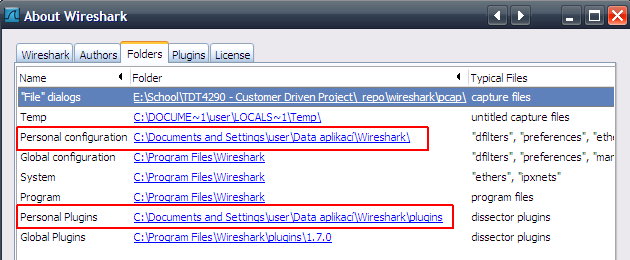
\includegraphics[width=\linewidth]{img/ws_about_folders.png}\hfill}
\begin{quote}
\begin{itemize}
\item {} 
on Linux/Unix system it may be  \code{\textasciitilde{}/.wireshark/} and  \code{\textasciitilde{}/.wireshark/plugins/}

\item {} 
on Windows it may be \code{C:\textbackslash{}Users\textbackslash{}*YourUserName*\textbackslash{}AppData\textbackslash{}Roaming\textbackslash{}Wireshark\textbackslash{}} 
and \code{C:\textbackslash{}Users\textbackslash{}*YourUserName*\textbackslash{}AppData\textbackslash{}Roaming\textbackslash{}Wireshark\textbackslash{}plugins\textbackslash{}}


\end{itemize}

If the folders does not exist, create them.
\end{quote}
\begin{enumerate}
\setcounter{enumi}{2}
\item {} 
Copy CSjark generated file \code{luastructs.lua} into the \code{Personal configuration} folder located in step 2.

\end{enumerate}

\begin{notice}{note}{Note:}
Location of CSjark generated files is given by \code{-o} command line argument. More in section {\hyperref[user/use:use]{\emph{Using CSjark}}}.
\end{notice}
\begin{enumerate}
\setcounter{enumi}{3}
\item {} 
Copy CSjark generated Lua dissector files into the \code{Personal Plugins} folder located in step 2.

\item {} 
Open the file \code{init.lua} located in the \code{Personal configuration} folder which you found in step 2. Insert the following code:

\begin{Verbatim}[commandchars=\\\{\}]
\PYG{n}{dofile}\PYG{p}{(}\PYG{l+s}{"}\PYG{l+s}{luastructs.lua}\PYG{l+s}{"}\PYG{p}{)}
\end{Verbatim}

\end{enumerate}
\begin{quote}

This ensures that the \code{luastructs.lua} is loaded before all other Lua scripts. \code{luastructs.lua} is a protocol that maps the id of the messages to the correct dissector, and calls them.
\end{quote}
\begin{enumerate}
\setcounter{enumi}{5}
\item {} 
Restart Wireshark. To check that the scripts are loaded, navigate to \code{Help} -\textgreater{} \code{About} -\textgreater{} \code{Plugins}. The scripts should now appear in the list as ``lua script''.



\end{enumerate}

{\hfill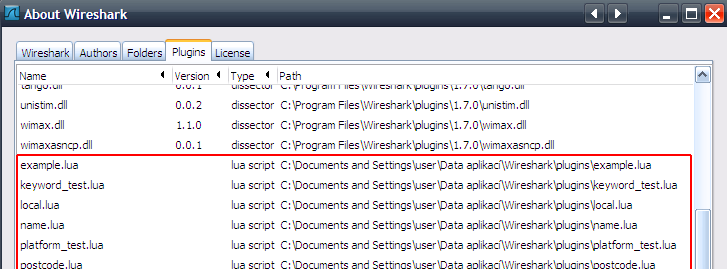
\includegraphics[width=\linewidth]{img/ws_about_plugins.png}\hfill}

To add further dissectors, only step 4, 5 and 6 needs to be repeated.

For further information on the Lua integration in Wireshark, please visit:
\href{http://www.wireshark.org/docs/wsug\_html\_chunked/wsluarm.html}{Lua Support in Wireshark}.


\section{Configuration}
\label{user/config:configuration}\label{user/config::doc}
Because there exists distinct requirements for flexibility of generating dissectors, CSjark supports configuration for various parts of the program. First, general parameters for utility running can be set up. This can be for example settings of variable sizes for different platforms or other parameters that could determine generating dissectors regardless actual C header file. Second, each individual C struct can be treated in different way. For example, value of specific struct member can be checked for being within specified limits.
\setbox0\vbox{
\begin{minipage}{0.95\linewidth}
\textbf{Contents}

\medskip

\begin{itemize}
\item {} 
{\hyperref[user/config:configuration]{Configuration}}
\begin{itemize}
\item {} 
{\hyperref[user/config:configuration-file-format-and-structure]{Configuration file format and structure}}

\item {} 
{\hyperref[user/config:struct-configuration]{Struct Configuration}}
\begin{itemize}
\item {} 
{\hyperref[user/config:value-ranges]{Value ranges}}

\item {} 
{\hyperref[user/config:value-explanations]{Value explanations}}
\begin{itemize}
\item {} 
{\hyperref[user/config:enums]{Enums}}

\item {} 
{\hyperref[user/config:bitstrings]{Bitstrings}}

\end{itemize}

\item {} 
{\hyperref[user/config:dissector-message-id]{Dissector message ID}}

\item {} 
{\hyperref[user/config:external-lua-dissectors]{External Lua dissectors}}
\begin{itemize}
\item {} 
{\hyperref[user/config:support-for-offset-and-value-in-lua-files]{Support for Offset and Value in Lua Files}}

\end{itemize}

\item {} 
{\hyperref[user/config:trailers]{Trailers}}

\item {} 
{\hyperref[user/config:custom-handling-of-data-types]{Custom handling of data types}}

\item {} 
{\hyperref[user/config:unknown-structs-handling]{Unknown structs handling}}

\end{itemize}

\item {} 
{\hyperref[user/config:options-configuration]{Options Configuration}}

\item {} 
{\hyperref[user/config:platform-specific-configuration]{Platform specific configuration}}

\end{itemize}

\end{itemize}
\end{minipage}}
\begin{center}\setlength{\fboxsep}{5pt}\shadowbox{\box0}\end{center}


\subsection{Configuration file format and structure}
\label{user/config:configuration-file-format-and-structure}\label{user/config:configfile}
\begin{notice}{note}{Note:}
Besides the configuration described below, one part of the configuration is held directly in the code. It represents the platform specific setup (file \code{platform.py}) - see {\hyperref[user/config:platform-specific-configuration]{Platform specific configuration}}.
\end{notice}

\textbf{Format}

The configuration files are written in \href{http://www.yaml.org/}{YAML} which is a data serialization format designed to be easy to read and write. The configuration must be put in a \code{.yml} file and specified when running CSjark as a command line argument (more about CLI in section {\hyperref[user/use:use]{\emph{Using CSjark}}}).

Basic YAML syntax is shown on following example:

\begin{Verbatim}[commandchars=\\\{\}]
\# comments can start anywhere with number sign (\#) and continues until the end of the line

key1: value1                   \# associative array of two key-value pairs
key2: value2                   \# pairs are separated by colon (:) and space ( ) on a separate line

\PYGZob{}key3: value3, key4: value4\PYGZcb{}   \# inline format of specifying associative arrays
                               \# pairs are separated by comma (,) and enclosed into curly braces (\PYGZob{}\PYGZcb{})

- item1                        \# list of two items
- item2                        \# each item starts with hyphen (-) and space ( ) on a separate line

[item3, item4]                 \# inline format of the list
                               \# items are separated by comma (,) and enclosed into square brackets ([])
\end{Verbatim}

Data structure hierarchy in YAML is maintained by outline indentation (whitespace is used, tab not allowed). All the basic elements can be combined to create a hierarchy:

\begin{Verbatim}[commandchars=\\\{\}]
Options:
    use\_cpp:                True
    generate\_placeholders:  True

Structs:
  - name:   struct1
    id:     [10, 12, 14]
  - name:   struct2
    id:     [11, 13, 15]
\end{Verbatim}

Strings are ordinarily unquoted, but may be enclosed in double-quotes (''), or single-quotes (`). The specific number of spaces in the indentation is unimportant as long as parallel elements have the same left justification and the hierarchically nested elements are indented further. This sample defines an associative array with 2 top level keys: one of the keys, ``Structs'', contains a 2 element array (or ``list''), each element of which is itself an associative array with differing keys.

Detailed specification of YAML syntax can be found at \href{http://www.yaml.org/spec/1.2/spec.html}{YAML website}.

\textbf{Structure}

CSjark configuration files might consist of two main parts:
\begin{itemize}
\item {} 
The first part is used for specifying all the configuration corresponding CSjark processing in general. More about CSjark options in {\hyperref[user/config:options-configuration]{Options Configuration}}.

\item {} 
The second part contains configuration for individual C struct definitions. That is described in section {\hyperref[user/config:struct-configuration]{Struct Configuration}}.

\end{itemize}

The configuration file may have following structure:

\begin{Verbatim}[commandchars=\\\{\}]
Options:
  \# there will be all your CSjark processing configuration
  use\_cpp: True
  ...

Structs:
  \# there will be a sequence of Struct definition configurations
  - name: struct1
    id: [10, 12, 14]
    \# another struct1 config
  - name: struct2
    id: [11, 13, 15]
    \# another struct2 config
\end{Verbatim}

\textbf{Automatic generation of configuration files}

Automatic generation of configuration file is a simple feature, that could save the user of the utility some time, since  the essential part of the configuration file is generated automatically.  The utility will only create a new file containing the name of the struct and line to specify the ID for the dissector.  To generate the configuration file, the utility must be run with \code{-p} or \code{-{-}placeholders} as an option (see {\hyperref[user/use:use]{\emph{Using CSjark}}} for more about CSjark CLI).


\subsection{Struct Configuration}
\label{user/config:struct-configuration}
Each individual C struct processed by CSjark can be treated in different way. All the configuration settings must be done in the \code{Structs} section of the configuration file. Every Struct definition is one item of the sequence and may contain these attributes:

\begin{tabulary}{\linewidth}{|L|L|}
\hline
\textbf{
Attribute name
} & \textbf{
Description
}\\\hline

name
 & 
C struct name (required field)
\\\hline

id
 & 
Dissector message id - more in {\hyperref[user/config:dissector-message-id]{Dissector message ID}}
\\\hline

description
 & 
Struct name displayed in Wireshark
\\\hline

size
 & 
Size of the struct in memory - more in {\hyperref[user/config:unknown-structs-handling]{Unknown structs handling}}
\\\hline

cnf
 & 
Conformance file name - more in {\hyperref[user/config:external-lua-dissectors]{External Lua dissectors}}
\\\hline

ranges
 & 
Value ranges limitations - more in {\hyperref[user/config:value-ranges]{Value ranges}}
\\\hline

enums
 & 
Enumeration definitions - more in {\hyperref[user/config:enums]{Enums}}
\\\hline

bitstrings
 & 
Bitstrings definitions - more in {\hyperref[user/config:bitstrings]{Bitstrings}}
\\\hline

trailers
 & 
Trailers definitions - more in {\hyperref[user/config:trailers]{Trailers}}
\\\hline

customs
 & 
Definitions for custom struct member handling - more in {\hyperref[user/config:custom-handling-of-data-types]{Custom handling of data types}}
\\\hline
\end{tabulary}


\textbf{General notes}
\begin{itemize}
\item {} 
Definition of \code{Structs} part of configuration is not mandatory. However, the user must be aware that if a struct configuration is not defined (namely the \code{id} attribute), it can be dissected only as a part of other struct (as its struct member). Otherwise there will be no dissectors registered for the struct.

\item {} 
If there exists a configuration for a struct member and also configuration for the type of this member, the behaviour is not defined. It is up to the user to ensure the definitions are exclusive for each struct member.
For example, in the {\hyperref[user/config:ranges]{\emph{Value ranges}}} section example, if the \code{percent} is defined as \emph{float}, the configuration would be ambiguous and there would be no guarantee that \code{percent} value is between 0 to 100 or -10 to 10.

\item {} 
If a struct contains another struct as its member, none of the configuration valid for the outer struct is applied on the nested struct. The same goes for unions. In order to configure the nested struct, the user must define separate struct configuration for it.
In this example, the configuration valid for the members of \emph{person} struct is not valid for members of \emph{address} struct

\begin{Verbatim}[commandchars=\\\{\}]
struct address \PYGZob{}
    int housenum;
    string street;
\PYGZcb{};

struct person \PYGZob{}
    string name;
    address adr;
    int age;
\PYGZcb{};
\end{Verbatim}

\end{itemize}


\subsubsection{Value ranges}
\label{user/config:ranges}\label{user/config:value-ranges}
Some variables may have a domain that is smaller than its given type. You could for example use an integer to describe percentage, which is a number between 0 and 100. It is possible to specify this to CSjark, so that the resulting dissector will tell Wireshark if the values are in the specified range or not. Value ranges are defined by the following syntax:

\begin{Verbatim}[commandchars=\\\{\}]
Structs:
  - name: "Name of the struct"
    id: 989
    ranges:
        - member \textbar{} type: "Name of struct member / type"
          min: "Lowest allowed value"
          max: "Highest allowed value"
\end{Verbatim}

When the definition specified as a type, the value range is applied to all the members of that type within the struct.

The value ranges configuration is valid only for data types that are meaningful for this purpose (e.g. integers, float, enums). Definitions for other data types are not taken into account.

Example:

\begin{Verbatim}[commandchars=\\\{\}]
Structs:
  - name: example\_struct
    id: 90
    ranges:
        - member: percent
          min: 0
          max: 100
        - type: float
          min: -10.0
          max: 10.0
\end{Verbatim}


\subsubsection{Value explanations}
\label{user/config:value-explanations}
Some variables may actually represent other values than its type. For example, for an enum it could be preferable to get the textual name of the value displayed, instead of the integer value that represent it. Such example can be an enum type or a bitstring.


\paragraph{Enums}
\label{user/config:enums}
Values of integer variables can be assigned to string values similarly to enumerated values in most programming languages. Thus, instead of integer value, a corresponding value defined in configuration file as a enumeration can be displayed.

The enumeration definition can be of two types. The first one, mapping specified integer by its struct member name, so it gains string value dependent on the actual integer value. And the second, where assigned string values correspond to every struct member of the type defined in the configuration.

The enum definition, as an attribute of the \code{Structs} item of the configuration file, always starts by \code{enums} keyword. It is followed by list of members/types for which we want to define enumerated integer values for. Each list item consists of 2 mandatory and 1 optional values

\begin{Verbatim}[commandchars=\\\{\}]
- member \textbar{} type: member name \textbar{} type name
  values: [value1, value2, ...] \textbar{} \PYGZob{} key1: value1, key2: value2, ...\PYGZcb{}
  strict: True \textbar{} False
\end{Verbatim}

where
\begin{itemize}
\item {} 
\code{member name}/\code{type name} contains string value of integer variable name for which we want to define enumerated values

\item {} 
\code{{[}value1, value2, ...{]}} is comma-separated list of enumerated values (implicitly numbered, starting from 0)

\item {} 
\code{\{ key1: value1, key2: value2, ...\}} is comma-separated list of key-value pairs, where \code{key} is integer value and \code{value} is it's assigned string value

\item {} 
\code{strict} is boolean value, which disables warning, if integer does not contain a value specified in the enum list (default \code{True})

\end{itemize}

Example of enums in struct definition contains:
- member named \code{weekday} and values defined as a list of key-value pairs.
- definition of enumerated values for \code{int} type. Values are given by simple list, therefore numbering is implicit (starting from 0, i.e. \code{Blue} = 2). Warning in case of invalid integer value \emph{will} be displayed.

\begin{Verbatim}[commandchars=\\\{\}]
Structs:
  - name: enum\_example1
    id: 10
    description: Enum config example
    enums:
      - member: weekday
        values: \PYGZob{}1: MONDAY, 2: TUESDAY, 3: WEDNESDAY, 4: THURSDAY, 5: FRIDAY, 6: SATURDAY, 7: SUNDAY\PYGZcb{}
      - type: int
        values: [Black, Red, Blue, Green, Yellow, White]
        strict: True \# Disable warning if not a valid value
\end{Verbatim}


\paragraph{Bitstrings}
\label{user/config:bitstrings}
It is possible to configure bitstrings in the utility. This makes it possible to view common data types like integer, short, float, etc. used as a bitstring in the wireshark dissector.

There is two ways to configure bitstrings, the first one is to specify a struct member and define the bit representation. The second option is to specify bits for all struct members of a given type.

These rules specifies the config:
\begin{itemize}
\item {} 
The bits are specified as 0...n, where 0 is the most significant bit

\item {} 
A bit group can be one or more bits.

\item {} 
Bit groups have a name

\item {} 
It is possible to name all possible values in a bit group.

\end{itemize}

Below, there is an example of a configuration for the member named \code{flags} and all the members of \code{short} type belonging to the struct \code{example}.
\begin{itemize}
\item {} 
member \code{flags}: This example has four bits specified, the first bit group is named ``In use'' and represent bit 0. The second group represent bit 1 and is named ``Endian'', and the values are named: 0 = ``Big'', 1 = ``Little''. The last group is ``Platform'' and represent bit 2-3 and have 4 named values.

\item {} 
type \code{short}: Each of the 3 bits represents one colour channel and it can be either ``True'' or ``False''.

\end{itemize}

\begin{Verbatim}[commandchars=\\\{\}]
Structs:
  - name: example
    id: 1000
    description: An example
    bitstrings:
      - member: flags
        0: In use
        1: [Endian, Big, Little]
        2-3: [Platform, Win, Linux, Mac, Solaris]
      - type: short
        0: Red
        1: Green
        2: Blue
\end{Verbatim}


\subsubsection{Dissector message ID}
\label{user/config:dissector-message-id}\label{user/config:ids}
Every packet with C struct captured by Wireshark contains a header. One of the fields in the header, the \code{id} field, specifies which dissector should be loaded to dissect the actual struct. The value of this field can be specified in the configuration file.

This is an example of the specification

\begin{Verbatim}[commandchars=\\\{\}]
Structs:
    - name: structname
      id: 10
\end{Verbatim}

More different messages can be dissected by one specific dissector. Therefore, the struct configuration can contain a whole list of dissector message ID's, that can process the struct.

\begin{Verbatim}[commandchars=\\\{\}]
Structs:
    - name: structname
      id: [12, 43, 3498]
\end{Verbatim}

\begin{notice}{note}{Note:}
The \code{id} must be an integer between 0 and 65535.
\end{notice}


\subsubsection{External Lua dissectors}
\label{user/config:external-lua-dissectors}
In some cases, CSjark will not be able to deliver the desired result from its own analysis, and the configuration options above may be too constraining. In this case, it is possible to write the lua dissector by hand, either for a given member or for an entire struct.

\begin{notice}{note}{Note:}
To be able to understand and write external Lua dissectors, the user should be familiar with basics of Lua programming and Lua integration into Wireshark.
More information how to write Lua code can be found in \href{http://www.lua.org/manual/5.1/}{Lua reference manual}. For further information on the Lua integration in Wireshark, please visit \href{http://www.Wireshark.org/docs/wsug\_html\_chunked/wsluarm.html}{Lua Support in Wireshark}.
\end{notice}

A custom Lua code for desired struct must be defined in an external conformance file with extension \code{.cnf}. The conformance file name and relative path then must be defined in the configuration file for the struct for which is the custom code applied for. The attribute name for the custom Lua definition file and path is \code{cnf}, as shown below:

\begin{Verbatim}[commandchars=\\\{\}]
\# CSjark configuration file

Structs:
    - name: custom\_lua
      cnf: etc/custom\_lua.cnf
      id: 1
      description: example of external custom Lua file definition
\end{Verbatim}

Writing the conformance file implies respecting following rules:
\begin{itemize}
\item {} 
Each section starts with \code{\#.\textless{}SECTION\textgreater{}} for example \code{\#.COMMENT}.

\item {} 
Unknown sections are ignored.

\end{itemize}

The conformance file implementation allows user to place the custom Lua code on various places within the Lua dissector code already generated by CSjark. There is a list of possible places:
\begin{quote}

\begin{tabulary}{\linewidth}{|L|L|}
\hline

\code{DEF\_HEADER id}
 & 
Lua code added before a Field definition.
\\\hline

\code{DEF\_BODY id}
 & 
Lua code to replace a Field definition. Within the definition, the original body can be referenced as \code{\%(DEFAULT\_BODY)s} or \code{\{DEFAULT\_BODY\}}
\\\hline

\code{DEF\_FOOTER id}
 & 
Lua code added after a Field definition
\\\hline

\code{DEF\_EXTRA}
 & 
Lua code added after the last definition
\\\hline

\code{FUNC\_HEADER id}
 & 
Lua code added before a Field function code
\\\hline

\code{FUNC\_BODY id}
 & 
Lua code to replace a Field function code
\\\hline

\code{FUNC\_FOOTER id}
 & 
Lua code added after a Field function code
\\\hline

\code{FUNC\_EXTRA}
 & 
Lua code added at end of dissector function
\\\hline

\code{COMMENT}
 & 
A multiline comment section
\\\hline

\code{END}
 & 
End of a section
\\\hline

\code{END\_OF\_CNF}
 & 
End of the conformance file
\\\hline
\end{tabulary}

\end{quote}

Where \code{id} denotes C struct member name . The \code{END} token is only optional, it does not have to be placed at the end of each section. However, all code after \code{END} token which is not part of another section defined above is discarded.

Example of such conformance file follows:

\begin{Verbatim}[commandchars=\\\{\}]
\#.COMMENT
    This is a .cnf file comment section
\#.END

\#.DEF\_HEADER super
-- This code will be added above the 'super' field definition
\#.END

\#.COMMENT
    DEF\_BODY replaces code inside the dissector function.
    Use \%(DEFAULT\_BODY)s or \PYGZob{}DEFAULT\_BODY\PYGZcb{} to use generated code.
\#.DEF\_BODY hyper
-- This is above 'hyper' definition
\%(DEFAULT\_BODY)s
-- This is below 'hyper'
\#.END

\#.DEF\_FOOTER name
-- This is below 'name' definition
\#.END

-- This text would be discarded.

\#.DEF\_EXTRA
-- This was all the Field definitions
\#.END


\#.FUNC\_HEADER precise
    -- This is above 'precise' inside the dissector function.
\#.END


\#.COMMENT
    FUNC\_BODY replaces code inside the dissector function.
    Use \%(DEFAULT\_BODY)s or \PYGZob{}DEFAULT\_BODY\PYGZcb{} to use generated code.
\#.FUNC\_BODY name
    --[[ This comments out the 'name' code
    \PYGZob{}DEFAULT\_BODY\PYGZcb{}
    ]]--
\#.END

\#.FUNC\_FOOTER super
    -- This is below 'super' inside dissector function
\#.END

\#.FUNC\_EXTRA
    -- This is the last line of the dissector function
\#.END\_OF\_CNF
\end{Verbatim}

This conformance file when run with this C header code:

\begin{Verbatim}[commandchars=\\\{\}]
struct custom\_lua \PYGZob{}
    short normal;
    int super;
    long long hyper;

    char name;
    double precise;

\PYGZcb{};
\end{Verbatim}

...will produce this Lua dissector:

\begin{Verbatim}[commandchars=\\\{\}]
-- Dissector for win32.custom\_lua: custom\_lua (Win32)
local proto\_custom\_lua = Proto("win32.custom\_lua", "custom\_lua (Win32)")

-- ProtoField definitions for: custom\_lua
local f = proto\_custom\_lua.fields
f.normal = ProtoField.int16("custom\_lua.normal", "normal")
-- This code will be added above the 'super' field definition
f.super = ProtoField.int32("custom\_lua.super", "super")
-- This is above 'hyper' definition
f.hyper = ProtoField.int64("custom\_lua.hyper", "hyper")
-- This is below 'hyper'
f.name = ProtoField.string("custom\_lua.name", "name")
-- This is below 'name' definition
f.precise = ProtoField.double("custom\_lua.precise", "precise")
-- This was all the field definitions

-- Dissector function for: custom\_lua
function proto\_custom\_lua.dissector(buffer, pinfo, tree)
    local subtree = tree:add\_le(proto\_custom\_lua, buffer())
    if pinfo.private.caller\_def\_name then
        subtree:set\_text(pinfo.private.caller\_def\_name .. ": " .. proto\_custom\_lua.description)
        pinfo.private.caller\_def\_name = nil
    else
        pinfo.cols.info:append(" (" .. proto\_custom\_lua.description .. ")")
    end

    subtree:add\_le(f.normal, buffer(0, 2))
    subtree:add\_le(f.super, buffer(4, 4))
    -- This is below 'super' inside dissector function
    subtree:add\_le(f.hyper, buffer(8, 8))
    --[[ This comments out the 'name' code
        subtree:add\_le(f.name, buffer(16, 1))
    ]]--
    -- This is above 'precise' inside the dissector function.
    subtree:add\_le(f.precise, buffer(24, 8))
    -- This is the last line of the dissector function
end

delegator\_register\_proto(proto\_custom\_lua, "Win32", "custom\_lua", 1)
\end{Verbatim}


\paragraph{Support for Offset and Value in Lua Files}
\label{user/config:support-for-offset-and-value-in-lua-files}
Via {\hyperref[user/config:external-lua-dissectors]{External Lua dissectors}} CSjark also provides a way to reference the proto fields of the dissector, with correct offset value and correct Lua variable.

To access the fields value and offset, \code{\{OFFSET\}} and \code{\{VALUE\}} strings may be put into the conformance file as shown below:

\begin{Verbatim}[commandchars=\\\{\}]
\#.FUNC\_FOOTER pointer
    -- Offset: \PYGZob{}OFFSET\PYGZcb{}
    -- Field value stored in lua variable: \PYGZob{}VALUE\PYGZcb{}
\#.END
\end{Verbatim}

Adding the offset and variable value is only possible in the parts that change the code of Lua functions, i.e. \code{FUNC\_HEADER}, \code{FUNC\_BODY} and \code{FUNC\_FOOTER}.

Above listed example leads to following Lua code:

\begin{Verbatim}[commandchars=\\\{\}]
local field\_value\_var = subtree:add(f.pointer, buffer(56,4))
    -- Offset: 56
    -- Field value stored in lua variable: field\_value\_var
\end{Verbatim}

\begin{notice}{note}{Note:}
The value of the referenced variable can be used after it is defined.
\end{notice}


\subsubsection{Trailers}
\label{user/config:trailers}
CSjark only creates dissectors from C structs defined as its input. To be able to use built-in dissectors in Wireshark, it is necessary to configure it. Wireshark has more than 1000 built-in dissectors. Several trailers can be configured for a packet.

The following parameters are allowed in trailers:
\begin{quote}

\begin{tabulary}{\linewidth}{|L|L|}
\hline

name
 & 
Protocol name for the built-in dissector
\\\hline

count
 & 
The number of trailers
\\\hline

member
 & 
Struct member, that contain the amount of trailers
\\\hline

size
 & 
Size of the buffer to feed to the protocol
\\\hline
\end{tabulary}

\end{quote}

There are two ways to configure the trailers - specify the total number of trailers or give a variable in the struct, which contains the amount of trailers. Both ways to configure trailers are shown below. In case the variable \code{trailer\_count} equals 2, the definitions has the same effect.

\begin{Verbatim}[commandchars=\\\{\}]
trailers:
  - name: proto1
    member: trailer\_count
    size: 32

trailers:
  - name: proto1
    count: 2
    size: 32
\end{Verbatim}

Example:
The example below shows an example with BER \footnote{
Basic Encoding Rules
}, which has 4 trailers with a size of 6 bytes.

\begin{Verbatim}[commandchars=\\\{\}]
trailers:
  - name: ber
  - count: 4
  - size: 6
\end{Verbatim}


\subsubsection{Custom handling of data types}
\label{user/config:custom-handling-of-data-types}
The utility supports custom handling of specified data types. Some variables in input C header may actually represent other values than its own type. This CSjark feature allows user to map types defined in C header to Wireshark field types. Also, it provides a method to change how the input field is displayed in Wireshark. The custom handling must be done through a configuration file.

For example, this functionality can cause Wireshark to display \code{time\_t} data type as \code{absolute\_time}. The displayed type is given by generated Lua dissector and functions of \code{ProtoField} class.

List of available output types follows:
\begin{description}
\item[{\code{Integer types}}] \leavevmode
uint8, uint16, uint24, uint32, uint64, int8, int16, int24, int32, int64, framenum

\item[{\code{Other types}}] \leavevmode
float, double, string, stringz, bytes, bool, ipv4, ipv6, ether, oid, guid, absolute\_time, relative\_time

\end{description}

For \code{Integer} types, there are some specific attributes that can be defined (see {\hyperref[user/config:below]{below}}). More about each individual type can be found in \href{http://www.Wireshark.org/docs/wsug\_html\_chunked/lua\_module\_Proto.html\#lua\_class\_ProtoField}{Wireshark reference}.

The section name in configuration file for custom data type handling is called \code{customs}. This section can contain following attributes:
\begin{itemize}
\item {} 
Required attributes
\begin{quote}

\begin{tabulary}{\linewidth}{|L|L|}
\hline
\textbf{
Attribute name
} & \textbf{
Value
}\\\hline

\code{member} \textbar{} \code{type}
 & 
Name of member or type for which is the configuration applied
\\\hline

\code{field}
 & 
Displayed type (see above)
\\\hline
\end{tabulary}

\end{quote}

\item {} 
Optional attributes - all types
\begin{quote}

\begin{tabulary}{\linewidth}{|L|L|}
\hline
\textbf{
Attribute name
} & \textbf{
Value
}\\\hline

\code{abbr}
 & 
Filter name of the field (the string that is used in filters)
\\\hline

\code{name}
 & 
Actual name of the field
\\\hline

\code{desc}
 & 
The description of the field (displayed on Wireshark statusbar)
\\\hline
\end{tabulary}

\end{quote}

\end{itemize}
\phantomsection\label{user/config:below}\begin{itemize}
\item {} 
Optional attributes - Integer types only:
\begin{quote}

\begin{tabulary}{\linewidth}{|L|L|}
\hline
\textbf{
Attribute name
} & \textbf{
Value
}\\\hline

\code{base}
 & 
Displayed representation - can be one of \code{base.DEC}, \code{base.HEX} or \code{base.OCT}
\\\hline

\code{values}
 & 
List of \code{key:value} pairs representing the Integer value - e.g. \code{\{0: Monday, 1: Tuesday\}}
\\\hline

\code{mask}
 & 
Integer mask of this field
\\\hline
\end{tabulary}

\end{quote}

\end{itemize}

Example of such a configuration file follows:

\begin{Verbatim}[commandchars=\\\{\}]
Structs:
  - name: custom\_type\_handling
    id: 1
    customs:
      - type: time\_t
        field: absolute\_time
      - member: day
        field: uint32
        abbr: day.name
        name: Weekday name
        base: base.DEC
        values: \PYGZob{} 0: Monday, 1: Tuesday, 2: Wednesday, 3: Thursday, 4: Friday\PYGZcb{}
        mask: nil
        desc: This day you will work a lot!!
\end{Verbatim}

and applies for example for this C header file:

\begin{Verbatim}[commandchars=\\\{\}]
\#include \textless{}time.h\textgreater{}

struct custom\_type\_handling \PYGZob{}
    time\_t abs;
    int day;
\PYGZcb{};
\end{Verbatim}

Both struct members are redefined. First will be displayed as \code{absolute\_type} according to its type (\code{time\_t}), second one is changed because of the struct member name (\code{day}).


\subsubsection{Unknown structs handling}
\label{user/config:unknown-structs-handling}
The header files that the utility parses, may have nested struct that is not defined in any other header file. To make  it possible to generate a dissector for this case, the user must be able to specify the size of the struct in a configuration file. When the sizes are specified it will be possible to generate a struct that can display the defined members of the struct correctly in the utility, for the parts that are not defined only the hex value will be displayed. This feature is added as a possible way to solve include dependencies that our utility is not able to solve. The user of the utility will get an error message when the utility is not able to find include dependencies, and the user may add the size of struct to be able to generate a dissector for the struct.

The size of unknown struct may be defined directly in the struct configuration as \code{size} attribute, similar to the example below:

\begin{Verbatim}[commandchars=\\\{\}]
Structs:
    - name: unknown struct
      id: 111
      size: 78
\end{Verbatim}

\begin{notice}{note}{Note:}
Size must be defined as a positive integer (or 0).
\end{notice}


\subsection{Options Configuration}
\label{user/config:options-configuration}
CSjark processing behaviour can be set up in various ways. Besides letting the user to specify how the CSjark should work by the command line arguments (see section {\hyperref[user/use:use]{\emph{Using CSjark}}}), it is also possible to define the options as a part of the configuration file(s).

\begin{tabulary}{\linewidth}{|L|L|L|L|}
\hline
\textbf{
Configuration file field
} & \textbf{
CLI equivalent
} & \textbf{
Value
} & \textbf{
Description
}\\\hline

\code{verbose}
 & 
\code{-v}
 & 
\code{True}/\code{False}
 & 
Print detailed information
\\\hline

\code{debug}
 & 
\code{-d}
 & 
\code{True}/\code{False}
 & 
Print debugging information
\\\hline

\code{strict}
 & 
\code{-s}
 & 
\code{True}/\code{False}
 & 
Only generate dissectors for known structs
\\\hline

\code{output\_dir}
 & 
\code{-o}
 & 
\code{None} or path
 & 
Definition of output destination
\\\hline

\code{output\_file}
 & 
\code{-o}
 & 
\code{None} or file name
 & 
Writes the output to the specified file
\\\hline

\code{generate\_placeholders}
 & 
\code{-p}
 & 
\code{True}/\code{False}
 & 
Generate placeholder config file for unknown structs
\\\hline

\code{use\_cpp}
 & 
\code{-n}
 & 
\code{True}/\code{False}
 & 
Enables/disables the C pre-processor
\\\hline

\code{cpp\_path}
 & 
\code{-C}
 & 
\code{None} or file name
 & 
Specifies which preprocessor to use
\\\hline

\code{excludes}
 & 
\code{-x}
 & 
List of excluded paths
 & 
File or folders to exclude from parsing
\\\hline

\code{platforms}
 &  & 
List of platform names
 & 
Set of platforms to support in dissectors
\\\hline

\code{include\_dirs}
 & 
\code{-I}
 & 
List of directories
 & 
Directories to be searched for Cpp includes
\\\hline

\code{includes}
 & 
\code{-i}
 & 
List of includes
 & 
Process file as Cpp \#include ``file'' directive
\\\hline

\code{defines}
 & 
\code{-D}
 & 
List of defines
 & 
Predefine name as a Cpp macro
\\\hline

\code{undefines}
 & 
\code{-U}
 & 
List of undefines
 & 
Cancel any previous Cpp definition of name
\\\hline

\code{arguments}
 & 
\code{-A}
 & 
List of additional arguments
 & 
Any additional C preprocessor arguments
\\\hline
\end{tabulary}


The last 5 options can be also specified separately for each individual input C header file. This can be achieved by adding sequence \code{files} with mandatory attribute \code{name}.

Below you can see an example of such \code{Options} section:

\begin{Verbatim}[commandchars=\\\{\}]
Options:
    verbose: True
    debug: False
    strict: False
    output\_dir: ../out
    output\_file: output.log
    generate\_placeholders: False
    use\_cpp: True
    cpp\_path: ../utils/cpp.exe
    excludes: [examples, test]
    platforms: [default, Win32, Win64, Solaris-sparc, Linux-x86]
    include\_dirs: [../more\_includes]
    includes: [foo.h, bar.h]
    defines: [CONFIG\_DEFINED=3, REMOVE=1]
    undefines: [REMOVE]
    arguments: [-D ARR=2]
    files:
      - name: a.h
        includes: [b.h, c.h]
        define: [MY\_DEFINE]
\end{Verbatim}

\begin{notice}{note}{Note:}
If you give CSjark multiple configuration files with the same values defined, it takes:
\begin{itemize}
\item {} 
for attributes with single value: a value from \emph{last processed config file} is valid

\item {} 
for attributes with list values: lists are \emph{merged}

\end{itemize}
\end{notice}


\subsection{Platform specific configuration}
\label{user/config:platform-specific-configuration}
To ensure that CSjark is usable as much as possible, platform specific

Entire platform setup is done via Python code, specifically \code{platform.py}. This file contains following sections:
\begin{enumerate}
\item {} 
Platform class definition including it's methods

\item {} 
Default mapping of C type and their Wireshark field type

\item {} 
Default C type size in bytes

\item {} 
Default alignment size in bytes

\item {} 
Custom C type sizes for every platform which differ from default

\item {} 
Custom alignment sizes for every platform which differ from default

\item {} 
Platform-specific C preprocessor macros

\item {} 
Platform registration method and calling for each platform

\end{enumerate}

When defining new platform, following steps should be done. Referenced sections apply to \code{platform.py} sections listed above. All the new dictionary variables should have proper syntax of \href{http://docs.python.org/release/3.1.3/tutorial/datastructures.html\#dictionaries}{Python dictionary}:
\begin{description}
\item[{\textbf{Field sizes}}] \leavevmode
Define custom C type sizes in section 5. Create new dictionary with name in capital letters. Only those different from default (section 3) must be defined.

\begin{Verbatim}[commandchars=\\\{\}]
\PYG{n}{NEW\PYGZus{}PLATFORM\PYGZus{}C\PYGZus{}SIZE\PYGZus{}MAP} \PYG{o}{=} \PYG{p}{\PYGZob{}}
    \PYG{l+s}{'}\PYG{l+s}{unsigned long}\PYG{l+s}{'}\PYG{p}{:} \PYG{l+m+mi}{8}\PYG{p}{,}
    \PYG{l+s}{'}\PYG{l+s}{unsigned long int}\PYG{l+s}{'}\PYG{p}{:} \PYG{l+m+mi}{8}\PYG{p}{,}
    \PYG{l+s}{'}\PYG{l+s}{long double}\PYG{l+s}{'}\PYG{p}{:} \PYG{l+m+mi}{16}
\PYG{p}{\PYGZcb{}}
\end{Verbatim}

\item[{\textbf{Memory alignment}}] \leavevmode
Define custom memory alignment sizes in section 6. Create new dictionary with name in capital letters. Only those different from default (section 4) must be defined.

\begin{Verbatim}[commandchars=\\\{\}]
\PYG{n}{NEW\PYGZus{}PLATFORM\PYGZus{}C\PYGZus{}ALIGNMENT\PYGZus{}MAP} \PYG{o}{=} \PYG{p}{\PYGZob{}}
    \PYG{l+s}{'}\PYG{l+s}{unsigned long}\PYG{l+s}{'}\PYG{p}{:} \PYG{l+m+mi}{8}\PYG{p}{,}
    \PYG{l+s}{'}\PYG{l+s}{unsigned long int}\PYG{l+s}{'}\PYG{p}{:} \PYG{l+m+mi}{8}\PYG{p}{,}
    \PYG{l+s}{'}\PYG{l+s}{long double}\PYG{l+s}{'}\PYG{p}{:} \PYG{l+m+mi}{16}
\PYG{p}{\PYGZcb{}}
\end{Verbatim}

\item[{\textbf{Macros}}] \leavevmode
Define dictionary of platform specific macros in section 7. These macros then can be used within C header files to define platform specific struct members etc. E.g.:

\begin{Verbatim}[commandchars=\\\{\}]
\#if \_WIN32
    float num;
\#elif \_\_sparc
    long double num;
\#else
    double num;
\end{Verbatim}

Example of such macros:

\begin{Verbatim}[commandchars=\\\{\}]
\PYG{n}{NEW\PYGZus{}PLATFORM\PYGZus{}MACROS} \PYG{o}{=} \PYG{p}{\PYGZob{}}
    \PYG{l+s}{'}\PYG{l+s}{\PYGZus{}\PYGZus{}new\PYGZus{}platform\PYGZus{}\PYGZus{}}\PYG{l+s}{'}\PYG{p}{:} \PYG{l+m+mi}{1}\PYG{p}{,} \PYG{l+s}{'}\PYG{l+s}{\PYGZus{}\PYGZus{}new\PYGZus{}platform}\PYG{l+s}{'}\PYG{p}{:} \PYG{l+m+mi}{1}
\PYG{p}{\PYGZcb{}}
\end{Verbatim}

\item[{\textbf{Register platform}}] \leavevmode
In last section (8), the new platform must be registered. Basically, it means calling the constructor of Platform class. That has following parameters:

\begin{Verbatim}[commandchars=\\\{\}]
\PYG{n}{Platform}\PYG{p}{(}\PYG{n}{name}\PYG{p}{,} \PYG{n}{flag}\PYG{p}{,} \PYG{n}{endian}\PYG{p}{,} \PYG{n}{macros}\PYG{o}{=}\PYG{n+nb+bp}{None}\PYG{p}{,} \PYG{n}{sizes}\PYG{o}{=}\PYG{n+nb+bp}{None}\PYG{p}{,} \PYG{n}{alignment}\PYG{o}{=}\PYG{n+nb+bp}{None}\PYG{p}{)}
\end{Verbatim}

where

\begin{tabulary}{\linewidth}{|L|L|}
\hline

\code{name}
 & 
name of the platform
\\\hline

\code{flag}
 & 
unique integer value representing this platform
\\\hline

\code{endian}
 & 
either \code{Platform.big} or \code{Platform.little}
\\\hline

\code{macros}
 & 
C preprocessor platform-specific macros like \_WIN32
\\\hline

\code{sizes}
 & 
dictionary which maps C types to their size in bytes
\\\hline
\end{tabulary}


Registering of the platform then might look as follows:

\begin{Verbatim}[commandchars=\\\{\}]
\PYG{c}{\PYGZsh{} New platform}
\PYG{n}{Platform}\PYG{p}{(}\PYG{l+s}{'}\PYG{l+s}{New-platform}\PYG{l+s}{'}\PYG{p}{,} \PYG{l+m+mi}{8}\PYG{p}{,} \PYG{n}{Platform}\PYG{o}{.}\PYG{n}{little}\PYG{p}{,}
         \PYG{n}{macros}\PYG{o}{=}\PYG{n}{NEW\PYGZus{}PLATFORM\PYGZus{}MACROS}\PYG{p}{,}
         \PYG{n}{sizes}\PYG{o}{=}\PYG{n}{NEW\PYGZus{}PLATFORM\PYGZus{}C\PYGZus{}SIZE\PYGZus{}MAP}\PYG{p}{,}
         \PYG{n}{alignment}\PYG{o}{=}\PYG{n}{NEW\PYGZus{}PLATFORM\PYGZus{}C\PYGZus{}ALIGNMENT\PYGZus{}MAP}\PYG{p}{)}
\end{Verbatim}

\end{description}


\chapter{Developer Documentation}
\label{index:yaml}\label{index:developer-documentation}

\section{Development rules}
\label{devel/general:development-rules}\label{devel/general::doc}
This document describes coding requirements and conventions for working with the CSjark code base. Please read it carefully and ask back any questions you might have.


\subsection{Coding Style Standard}
\label{devel/general:coding-style-standard}
The programming language used to implement the utility is Python. All the code should as much as possible follow the coding style described in the Style Guide for Python Code (\href{http://www.python.org/dev/peps/pep-0008/}{PEP8}). In addition we decided that the design should attempt to be pythonic, as detailed by \href{http://www.python.org/dev/peps/pep-0020/}{PEP20}.


\subsection{Code base}
\label{devel/general:pep20}\label{devel/general:code-base}
The entire CSjark project is hosted on \href{https://github.com/}{GitHub}. In order to get the source code, you can:
\begin{itemize}
\item {} 
clone the Git repository: \href{https://github.com/eventh/kpro9}{https://github.com/eventh/kpro9}

\item {} 
\href{https://github.com/eventh/kpro9/zipball/master}{download most recent tar archive}

\item {} 
\href{https://github.com/eventh/kpro9/tarball/master}{download most recent zip archive}

\end{itemize}

\begin{notice}{note}{Note:}
When commiting to the repository, always write good log messages. It will help people that will read the diffs in the future.
\end{notice}


\subsection{Issue tracking}
\label{devel/general:issue-tracking}
For issue tracking, we use bug tracking capabilities of GitHub. You can register bugs, discuss issues or see what’s going on for the next milestone, both from an email and from a web interface.

\href{https://github.com/eventh/kpro9/issues}{https://github.com/eventh/kpro9/issues}


\section{Design Overview}
\label{devel/design::doc}\label{devel/design:design-overview}
This part describes the design of the CSjark to help all the future developers to understand what is under the hood.


\subsection{Textual description}
\label{devel/design:textual-description}
CSjark starts with the \emph{csjark} module. It takes as input command line arguments, including file and folder names for C header files and configuration files.
It replaces folder names with the file names of the files inside the folders, and checks that all the files exists, then it gives the names of the configuration files to the \emph{config} module.

The \emph{config} module parses configuration files and stores them in suitable config data structures in memory. It takes as input file names, and it opens those files to read their content.

\emph{Csjark} module then gives file names of C header files to the \emph{cpp} module. The \emph{cpp} module gives the file names and some other arguments to an external program, the C preprocessor (\emph{cpp.exe} on Windows). This external program opens the header files, and when it encounters \emph{\#include} directives it searches for the right file and opens it as well. The output of this external program is just a long string of C code, which \emph{cpp} module returns to the \emph{csjark} module.

The \emph{csjark} module then gives the C code string to \emph{cparser} module, which forwards the string to pycparser. Pycparser parse the C code to generate an abstract syntax tree, which it returns to \emph{cparser} which returns it to \emph{csjark}.

Csjark module then tells \emph{cparser} to find all struct definitions in the abstract syntax tree, which it does by traversing the tree. Each time it finds a struct, it asks \emph{dissector} module to create a protocol for it. Afterwards \emph{cparser} holds a list of all the created protocols.

Csjark then gets the list of protocols from \emph{cparser}, and for each one asks \emph{dissector} module to generate lua code for Wireshark dissectors. It writes these dissectors to files, and finishes with a status message informing the user how it all went.

The new \emph{field} module is simply to move class \emph{Fields} and its sub-classes into their own module to make \emph{dissector} module smaller and less complex.

\textbf{Summary}

\emph{csjark} module writes Lua files, \emph{config} module opens and reads YAML files, \emph{cpp} module starts an external program which reads C header files. The structure as well as the associations among the classes are shown on following {\hyperref[devel/design:module]{module}} and {\hyperref[devel/design:class]{class}} diagrams.


\subsection{Module diagram}
\label{devel/design:module-diagram}\label{devel/design:module}\begin{figure}[htbp]
\centering
\capstart

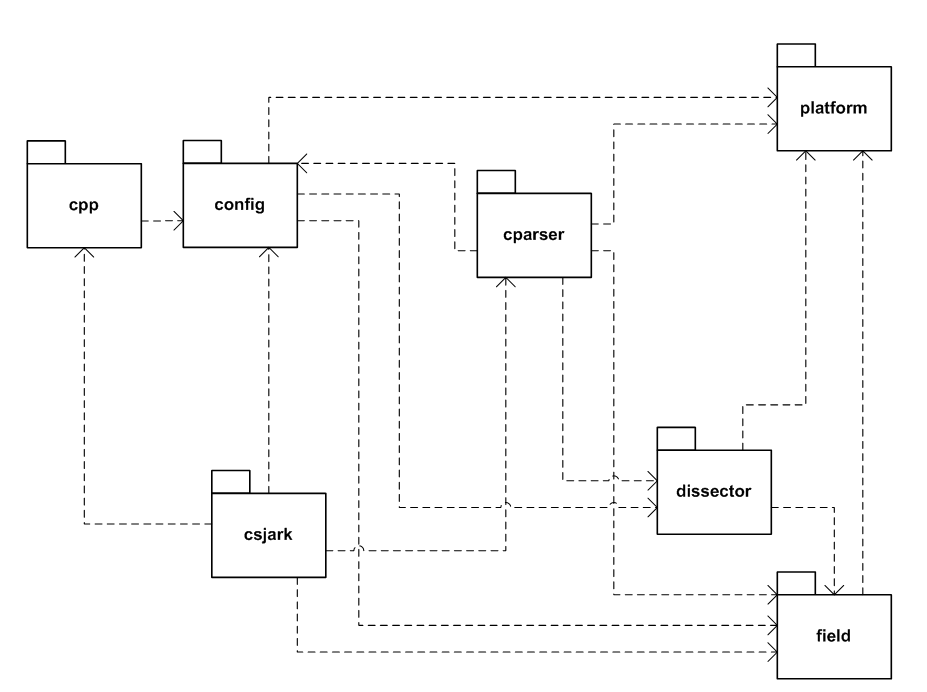
\includegraphics[width=0.600\linewidth]{img/module_diagram.png}
\caption{\emph{CSjark: module diagram}}\end{figure}


\subsection{Class diagram}
\label{devel/design:class-diagram}\label{devel/design:class}\begin{figure}[htbp]
\centering
\capstart

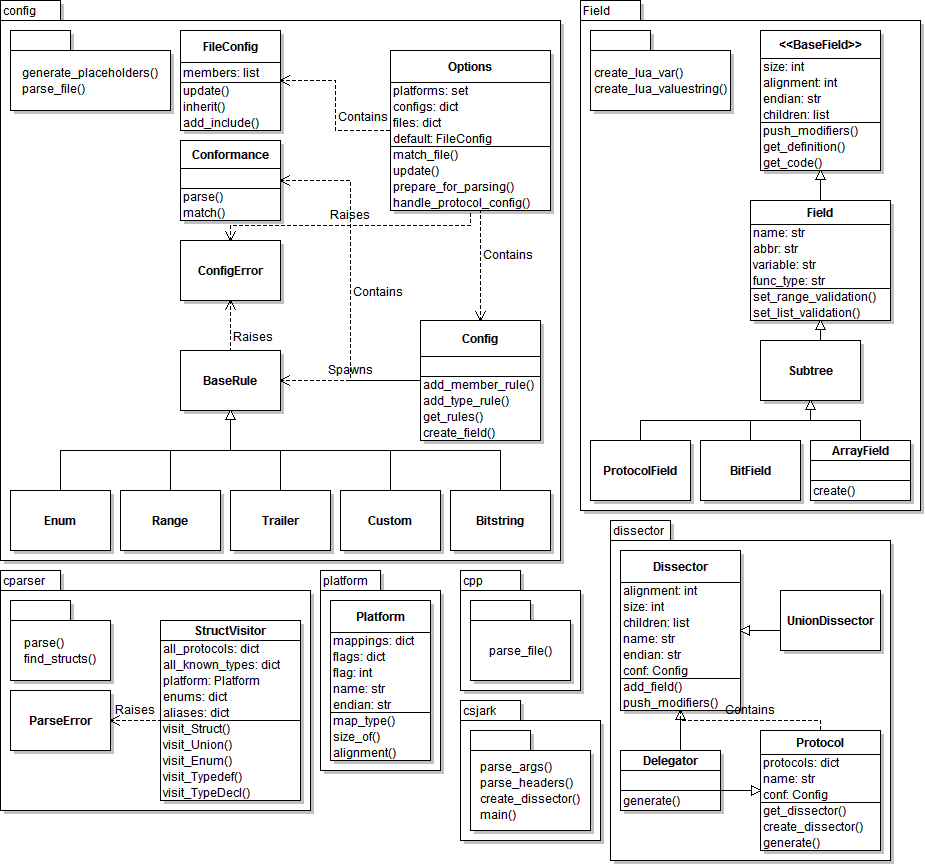
\includegraphics[width=\linewidth]{img/class_diagram.png}
\caption{\emph{CSjark: class diagram}}\end{figure}


\section{Testing}
\label{devel/testing:testing}\label{devel/testing::doc}
There are several types of tests done for verification of CSjark functionality:


\subsection{White box testing}
\label{devel/testing:white-box-testing}
This type of white box testing basically means verification of functionality of specific section of the code, usually at the function level. As a tool for creating white box unit tests, the team decided to use the \href{http://packages.python.org/Attest/}{Attest} testing framework for python code.


\subsection{Black box testing}
\label{devel/testing:black-box-testing}
In general black box testing does not require the tester to have any intimate knowledge about the system or any of the programming logic that went into making it. Black box test cases are built around the specifications and requirements of a system, for example its functional, and in some cases, non-functional requirements.

For CSjark, black box testing means feeding the utility with input C header file, corresponding configuration file and generating the output (Lua dissector). Then, the generated output is compared to expected output.

Another way how to do the black box testing to use the generated dissectors in Wireshark. For this purpose, we also need a \code{pcap} file containing the IPC packets that corresponds to the input C header files. You can read more about whole process in the User Manual section {\hyperref[user/intro:intro]{\emph{Introduction}}}. A short guide how to create \code{pcap} file for the C struct can be found in the \href{https://github.com/eventh/kpro9/wiki/text2pcap}{project wiki}.

With the generated Lua dissectors, it should possible to display the contents of the C struct within the IPC packets. Also, according to the utility requirements, it should be possible to filter and search by any variable name or its value. This way of testing is based on manual checking of the individual variable values. The process involves several manual steps and therefore cannot be automated.


\subsection{Regression testing}
\label{devel/testing:project-wiki}\label{devel/testing:regression-testing}
The test must be written in a way that it should be possible to run them repeatedly after the first run. That can ensure that all the implemented functionality is still working well after changes in the code.


\subsection{Creating tests}
\label{devel/testing:creating-tests}
To create tests using Attest, you start by importing \code{Tests}, \code{assert\_hook} and optionally \code{contexts} from \code{attest} library. You then create a variable and initialize it to an instance of Tests, which is the variable that will contain list functions that each constitutes one test that is to be run. To feed your test instance with functions for testing you then have to mark these functions with a decorator and feed it the \code{.tests} function of the Tests instance. After creating a unit test in this fashion you can run all of your unit tests through Attest from the command line by typing:

\begin{Verbatim}[commandchars=\\\{\}]
python -m attest
\end{Verbatim}

This runs all of your unit tests through Attest and returns a message telling the user how many assertions failed, as well as what input made them fail. For more information read the user documentation of \href{http://packages.python.org/Attest/}{Attest}.


\subsection{Testing code}
\label{devel/testing:attest}\label{devel/testing:testing-code}
All the test code, the testing configuration files and the testing input files are located in folder
\begin{quote}

\href{https://github.com/eventh/kpro9/tree/master/CSjark/csjark/test}{CSjark/csjark/test}
\end{quote}

It contains modules for unit/module testing of each of the CSjark modules as well as modules for bundled white/black box testing.


\section{Source code overview}
\label{devel/code::doc}\label{devel/code:source-code-overview}
\textbf{Program modules}

\begin{longtable}{ll}
\hline
\endfirsthead

\multicolumn{2}{c}%
{{\bfseries \tablename\ \thetable{} -- continued from previous page}} \\
\hline
\endhead

\hline \multicolumn{2}{|r|}{{Continued on next page}} \\ \hline
\endfoot

\hline
\endlastfoot


{\hyperref[devel/code:module-csjark]{\code{csjark}}}
 & 
CSjark is a tool for generating Lua dissectors from C struct
\\\hline

{\hyperref[devel/code:module-config]{\code{config}}}
 & 
A module for configuration of our utility.
\\\hline

{\hyperref[devel/code:module-cpp]{\code{cpp}}}
 & 
Module for performing the C preprocessor step on C header files.
\\\hline

{\hyperref[devel/code:module-cparser]{\code{cparser}}}
 & 
A module for parsing C files to find struct definitions.
\\\hline

{\hyperref[devel/code:module-field]{\code{field}}}
 & 
A module for classes which represents values in a packet.
\\\hline

{\hyperref[devel/code:module-dissector]{\code{dissector}}}
 & 
A module for generating Lua dissectors for Wireshark.
\\\hline

{\hyperref[devel/code:module-platform]{\code{platform}}}
 & 
A module which holds platform specific configuration.
\\\hline
\end{longtable}


\textbf{Testing modules}

Modules for testing are located in
\begin{quote}

\href{https://github.com/eventh/kpro9/tree/master/CSjark/csjark/test}{CSjark/csjark/test}
\end{quote}


\subsection{csjark}
\label{devel/code:csjark}\label{devel/code:module-csjark}\index{csjark (module)}
CSjark is a tool for generating Lua dissectors from C struct
definitions to use with Wireshark.
\begin{description}
\item[{usage: csjark.py {[}-h{]} {[}-v{]} {[}-d{]} {[}-s{]} {[}-f {[}header {[}header ...{]}{]}{]}}] \leavevmode
{[}-c {[}config {[}config ...{]}{]}{]} {[}-x {[}path {[}path ...{]}{]}{]}
{[}-o {[}output{]}{]} {[}-p{]} {[}-n{]} {[}-C {[}cpp{]}{]} {[}-i {[}header {[}header ...{]}{]}{]}
{[}-I {[}directory {[}directory ...{]}{]}{]}
{[}-D {[}name=definition {[}name=definition ...{]}{]}{]}
{[}-U {[}name {[}name ...{]}{]}{]} {[}-A {[}argument {[}argument ...{]}{]}{]}
{[}header{]} {[}config{]}

\end{description}

Generate Wireshark dissectors from C structs.
\begin{description}
\item[{positional arguments:}] \leavevmode
header                C header file to parse
config                yaml config file to parse

\item[{optional arguments:}] \leavevmode\begin{optionlist}{3cm}
\item [-h, -{-}help]  
show this help message and exit
\item [-v, -{-}verbose]  
print detailed information
\item [-d, -{-}debug]  
print debugging information
\item [-s, -{-}strict]  
only generate dissectors for known structs
\item [-n, -{-}nocpp]  
disable C preprocessor
\item [-p, -{-}placeholders]  
generate placeholder config file for unknown structs
\item [-f, -{-}file]  
C header or code file(s) to parse
\item [-c, -{-}config]  
configuration file(s) to parse
\item [-x, -{-}exclude]  
file or folders to exclude from parsing
\item [-o, -{-}output]  
write output to directory/file
\item [-C, -{-}Cpppath]  
which C preprocessor to use
\item [-i, -{-}include]  
process file as Cpp \#include ``file'' directive
\item [-I, -{-}Includes]  
directories to be searched for Cpp includes
\item [-D, -{-}Define]  
predefine name as a Cpp macro
\item [-U, -{-}Undefine]  
cancel any previous Cpp definition of name
\item [-A, -{-}Additional]  
any additional C preprocessor arguments
\end{optionlist}

\end{description}

Example:
``python csjark.py -v --nocpp headerfile.h configfile.yml''
\index{parse\_args() (in module csjark)}

\begin{fulllineitems}
\phantomsection\label{devel/code:csjark.parse_args}\pysiglinewithargsret{\code{csjark.}\bfcode{parse\_args}}{\emph{args=None}}{}
Parse arguments given in sys.argv.

`args' is a list of strings to parse instead of sys.argv.

\end{fulllineitems}

\index{parse\_headers() (in module csjark)}

\begin{fulllineitems}
\phantomsection\label{devel/code:csjark.parse_headers}\pysiglinewithargsret{\code{csjark.}\bfcode{parse\_headers}}{\emph{headers}}{}
Parse `headers' to create a Wireshark protocol dissector.

\end{fulllineitems}

\index{create\_dissector() (in module csjark)}

\begin{fulllineitems}
\phantomsection\label{devel/code:csjark.create_dissector}\pysiglinewithargsret{\code{csjark.}\bfcode{create\_dissector}}{\emph{filename}, \emph{platform}, \emph{folders=None}, \emph{includes=None}}{}
Parse `filename' to create a Wireshark protocol dissector.

`filename' is the C header/code file to parse.
`platform' is the platform we should simulate.
`folders' is a set of all folders to -Include.
`includes' is a set of filenames to \#include.
Returns the error if parsing failed, None if succeeded.

\end{fulllineitems}

\index{\_write\_dissector() (in module csjark)}

\begin{fulllineitems}
\phantomsection\label{devel/code:csjark._write_dissector}\pysiglinewithargsret{\code{csjark.}\bfcode{\_write\_dissector}}{\emph{name}, \emph{proto}}{}
Write a single dissector to file.

\end{fulllineitems}

\index{write\_dissectors\_to\_file() (in module csjark)}

\begin{fulllineitems}
\phantomsection\label{devel/code:csjark.write_dissectors_to_file}\pysiglinewithargsret{\code{csjark.}\bfcode{write\_dissectors\_to\_file}}{\emph{all\_protocols}}{}
Write lua dissectors to file(s).

\end{fulllineitems}

\index{write\_delegator\_to\_file() (in module csjark)}

\begin{fulllineitems}
\phantomsection\label{devel/code:csjark.write_delegator_to_file}\pysiglinewithargsret{\code{csjark.}\bfcode{write\_delegator\_to\_file}}{}{}
Write the lua file which delegates dissecting to dissectors.

\end{fulllineitems}

\index{write\_placeholders\_to\_file() (in module csjark)}

\begin{fulllineitems}
\phantomsection\label{devel/code:csjark.write_placeholders_to_file}\pysiglinewithargsret{\code{csjark.}\bfcode{write\_placeholders\_to\_file}}{\emph{protocols}}{}
Write a placeholder file for `protocols' with no configuration.

\end{fulllineitems}

\index{main() (in module csjark)}

\begin{fulllineitems}
\phantomsection\label{devel/code:csjark.main}\pysiglinewithargsret{\code{csjark.}\bfcode{main}}{}{}
Run the CSjark program.

\end{fulllineitems}



\subsection{config}
\label{devel/code:module-config}\label{devel/code:config}\index{config (module)}
A module for configuration of our utility.

Should parse config files and create data structures which the parser can
use when translating C struct definitions to Wireshark protocols and fields.

Config class holds configuration for specific struct by name. FileConfig
holds C preprocessor options for specific files by path. Options holds
global utility configuration, include dictinaries for the Config and
Fileconfig instances.

Additionally there is the BaseRule class and its subclasses which holds
specific rules specified by configuration for members in structs.
\index{ConfigError}

\begin{fulllineitems}
\phantomsection\label{devel/code:config.ConfigError}\pysigline{\strong{exception }\code{config.}\bfcode{ConfigError}}
Exception raised by invalid configuration.

\end{fulllineitems}

\index{Config (class in config)}

\begin{fulllineitems}
\phantomsection\label{devel/code:config.Config}\pysiglinewithargsret{\strong{class }\code{config.}\bfcode{Config}}{\emph{name}}{}
Holds configuration for a specific protocol.
\index{add\_member\_rule() (config.Config method)}

\begin{fulllineitems}
\phantomsection\label{devel/code:config.Config.add_member_rule}\pysiglinewithargsret{\bfcode{add\_member\_rule}}{\emph{member}, \emph{rule}}{}
Add a new rule for a specific member.

`member' is the member of a struct to match
`rule' is the new rule to add

\end{fulllineitems}

\index{add\_type\_rule() (config.Config method)}

\begin{fulllineitems}
\phantomsection\label{devel/code:config.Config.add_type_rule}\pysiglinewithargsret{\bfcode{add\_type\_rule}}{\emph{type}, \emph{rule}}{}
Add a new rule for all members of a specific type.

`type' is the C type to match members against
`rule' is the new rule to add

\end{fulllineitems}

\index{get\_rules() (config.Config method)}

\begin{fulllineitems}
\phantomsection\label{devel/code:config.Config.get_rules}\pysiglinewithargsret{\bfcode{get\_rules}}{\emph{member}, \emph{type}}{}
Return all rules which match `member' or `type'.

\end{fulllineitems}

\index{create\_field() (config.Config method)}

\begin{fulllineitems}
\phantomsection\label{devel/code:config.Config.create_field}\pysiglinewithargsret{\bfcode{create\_field}}{\emph{proto}, \emph{name}, \emph{ctype}, \emph{size}, \emph{alignment}, \emph{endian}}{}
Create a field depending on rules.

\end{fulllineitems}


\end{fulllineitems}

\index{BaseRule (class in config)}

\begin{fulllineitems}
\phantomsection\label{devel/code:config.BaseRule}\pysiglinewithargsret{\strong{class }\code{config.}\bfcode{BaseRule}}{\emph{conf}, \emph{obj}}{}
A base class for rules referring to protocol fields.

\end{fulllineitems}

\index{Range (class in config)}

\begin{fulllineitems}
\phantomsection\label{devel/code:config.Range}\pysiglinewithargsret{\strong{class }\code{config.}\bfcode{Range}}{\emph{conf}, \emph{obj}}{}
Rule for specifying a valid range for a member or type.

\end{fulllineitems}

\index{Enum (class in config)}

\begin{fulllineitems}
\phantomsection\label{devel/code:config.Enum}\pysiglinewithargsret{\strong{class }\code{config.}\bfcode{Enum}}{\emph{conf}, \emph{obj}}{}
Rule for emulating enum with int-like types.

\end{fulllineitems}

\index{Bitstring (class in config)}

\begin{fulllineitems}
\phantomsection\label{devel/code:config.Bitstring}\pysiglinewithargsret{\strong{class }\code{config.}\bfcode{Bitstring}}{\emph{conf}, \emph{obj}}{}
Rule for representing ints which are bit strings.

\end{fulllineitems}

\index{Trailer (class in config)}

\begin{fulllineitems}
\phantomsection\label{devel/code:config.Trailer}\pysiglinewithargsret{\strong{class }\code{config.}\bfcode{Trailer}}{\emph{conf}, \emph{obj}}{}
Rule for specifying one or more trailer protocol(s).

\end{fulllineitems}

\index{Custom (class in config)}

\begin{fulllineitems}
\phantomsection\label{devel/code:config.Custom}\pysiglinewithargsret{\strong{class }\code{config.}\bfcode{Custom}}{\emph{conf}, \emph{obj}}{}
Rule for specifying a custom field handling.
\index{create() (config.Custom method)}

\begin{fulllineitems}
\phantomsection\label{devel/code:config.Custom.create}\pysiglinewithargsret{\bfcode{create}}{\emph{proto}, \emph{name}, \emph{ctype}, \emph{size}, \emph{alignment}, \emph{endian}}{}
Create a new Field based on this rule.

\end{fulllineitems}


\end{fulllineitems}

\index{ConformanceFile (class in config)}

\begin{fulllineitems}
\phantomsection\label{devel/code:config.ConformanceFile}\pysiglinewithargsret{\strong{class }\code{config.}\bfcode{ConformanceFile}}{\emph{conf}, \emph{file}, \emph{config\_file='`}}{}
A class for parsing a conformance file.

A conformance file specifies custom lua code for fields.
It can give custom code for the definition, and inside the dissector
function. For these two cases, it supports header, body, footer and
extra sections which places code above, instead of, below, or at the
end of the section.

Each section starts with \#.\textless{}SECTION\textgreater{} for example \#.COMMENT.
Unknown sections are ignore, to be compatible with Asn2wrs .cnf files.
\index{t\_def\_hdr (config.ConformanceFile attribute)}

\begin{fulllineitems}
\phantomsection\label{devel/code:config.ConformanceFile.t_def_hdr}\pysigline{\bfcode{t\_def\_hdr}\strong{ = `DEF\_HEADER'}}
\end{fulllineitems}

\index{t\_def\_body (config.ConformanceFile attribute)}

\begin{fulllineitems}
\phantomsection\label{devel/code:config.ConformanceFile.t_def_body}\pysigline{\bfcode{t\_def\_body}\strong{ = `DEF\_BODY'}}
\end{fulllineitems}

\index{t\_def\_ftr (config.ConformanceFile attribute)}

\begin{fulllineitems}
\phantomsection\label{devel/code:config.ConformanceFile.t_def_ftr}\pysigline{\bfcode{t\_def\_ftr}\strong{ = `DEF\_FOOTER'}}
\end{fulllineitems}

\index{t\_def\_extra (config.ConformanceFile attribute)}

\begin{fulllineitems}
\phantomsection\label{devel/code:config.ConformanceFile.t_def_extra}\pysigline{\bfcode{t\_def\_extra}\strong{ = `DEF\_EXTRA'}}
\end{fulllineitems}

\index{t\_func\_hdr (config.ConformanceFile attribute)}

\begin{fulllineitems}
\phantomsection\label{devel/code:config.ConformanceFile.t_func_hdr}\pysigline{\bfcode{t\_func\_hdr}\strong{ = `FUNC\_HEADER'}}
\end{fulllineitems}

\index{t\_func\_body (config.ConformanceFile attribute)}

\begin{fulllineitems}
\phantomsection\label{devel/code:config.ConformanceFile.t_func_body}\pysigline{\bfcode{t\_func\_body}\strong{ = `FUNC\_BODY'}}
\end{fulllineitems}

\index{t\_func\_ftr (config.ConformanceFile attribute)}

\begin{fulllineitems}
\phantomsection\label{devel/code:config.ConformanceFile.t_func_ftr}\pysigline{\bfcode{t\_func\_ftr}\strong{ = `FUNC\_FOOTER'}}
\end{fulllineitems}

\index{t\_func\_extra (config.ConformanceFile attribute)}

\begin{fulllineitems}
\phantomsection\label{devel/code:config.ConformanceFile.t_func_extra}\pysigline{\bfcode{t\_func\_extra}\strong{ = `FUNC\_EXTRA'}}
\end{fulllineitems}

\index{t\_comment (config.ConformanceFile attribute)}

\begin{fulllineitems}
\phantomsection\label{devel/code:config.ConformanceFile.t_comment}\pysigline{\bfcode{t\_comment}\strong{ = `COMMENT'}}
\end{fulllineitems}

\index{t\_end (config.ConformanceFile attribute)}

\begin{fulllineitems}
\phantomsection\label{devel/code:config.ConformanceFile.t_end}\pysigline{\bfcode{t\_end}\strong{ = `END'}}
\end{fulllineitems}

\index{t\_end\_cnf (config.ConformanceFile attribute)}

\begin{fulllineitems}
\phantomsection\label{devel/code:config.ConformanceFile.t_end_cnf}\pysigline{\bfcode{t\_end\_cnf}\strong{ = `END\_OF\_CNF'}}
\end{fulllineitems}

\index{def\_tokens (config.ConformanceFile attribute)}

\begin{fulllineitems}
\phantomsection\label{devel/code:config.ConformanceFile.def_tokens}\pysigline{\bfcode{def\_tokens}\strong{ = {[}'DEF\_HEADER', `DEF\_BODY', `DEF\_FOOTER'{]}}}
\end{fulllineitems}

\index{func\_tokens (config.ConformanceFile attribute)}

\begin{fulllineitems}
\phantomsection\label{devel/code:config.ConformanceFile.func_tokens}\pysigline{\bfcode{func\_tokens}\strong{ = {[}'FUNC\_HEADER', `FUNC\_BODY', `FUNC\_FOOTER'{]}}}
\end{fulllineitems}

\index{store\_tokens (config.ConformanceFile attribute)}

\begin{fulllineitems}
\phantomsection\label{devel/code:config.ConformanceFile.store_tokens}\pysigline{\bfcode{store\_tokens}\strong{ = {[}'DEF\_HEADER', `DEF\_BODY', `DEF\_FOOTER', `FUNC\_HEADER', `FUNC\_BODY', `FUNC\_FOOTER', `DEF\_EXTRA', `FUNC\_EXTRA'{]}}}
\end{fulllineitems}

\index{valid\_tokens (config.ConformanceFile attribute)}

\begin{fulllineitems}
\phantomsection\label{devel/code:config.ConformanceFile.valid_tokens}\pysigline{\bfcode{valid\_tokens}\strong{ = {[}'DEF\_HEADER', `DEF\_BODY', `DEF\_FOOTER', `FUNC\_HEADER', `FUNC\_BODY', `FUNC\_FOOTER', `DEF\_EXTRA', `FUNC\_EXTRA', `COMMENT', `END', `END\_OF\_CNF'{]}}}
\end{fulllineitems}

\index{\_get\_token() (config.ConformanceFile method)}

\begin{fulllineitems}
\phantomsection\label{devel/code:config.ConformanceFile._get_token}\pysiglinewithargsret{\bfcode{\_get\_token}}{\emph{line}}{}
Find the token and the field it refers to.

\end{fulllineitems}

\index{parse() (config.ConformanceFile method)}

\begin{fulllineitems}
\phantomsection\label{devel/code:config.ConformanceFile.parse}\pysiglinewithargsret{\bfcode{parse}}{}{}
Parse the conformance file's sections and content.

\end{fulllineitems}

\index{match() (config.ConformanceFile method)}

\begin{fulllineitems}
\phantomsection\label{devel/code:config.ConformanceFile.match}\pysiglinewithargsret{\bfcode{match}}{\emph{name}, \emph{code}, \emph{definition=False}, \emph{field=None}}{}
Modify fields code if a cnf file demands it.

\end{fulllineitems}


\end{fulllineitems}

\index{FileConfig (class in config)}

\begin{fulllineitems}
\phantomsection\label{devel/code:config.FileConfig}\pysiglinewithargsret{\strong{class }\code{config.}\bfcode{FileConfig}}{\emph{name}}{}
Holds options for specific files.
\index{members (config.FileConfig attribute)}

\begin{fulllineitems}
\phantomsection\label{devel/code:config.FileConfig.members}\pysigline{\bfcode{members}\strong{ = (`include\_dirs', `includes', `defines', `undefines', `arguments')}}
\end{fulllineitems}

\index{update() (config.FileConfig method)}

\begin{fulllineitems}
\phantomsection\label{devel/code:config.FileConfig.update}\pysiglinewithargsret{\bfcode{update}}{\emph{obj}}{}
Update variables with config from a yml file.

\end{fulllineitems}

\index{inherit() (config.FileConfig method)}

\begin{fulllineitems}
\phantomsection\label{devel/code:config.FileConfig.inherit}\pysiglinewithargsret{\bfcode{inherit}}{\emph{parent}}{}
Update variables with config from another FileConfig instance.

\end{fulllineitems}

\index{add\_include() (config.FileConfig class method)}

\begin{fulllineitems}
\phantomsection\label{devel/code:config.FileConfig.add_include}\pysiglinewithargsret{\strong{classmethod }\bfcode{add\_include}}{\emph{filename}, \emph{include}}{}
Add a new `include' to `filename' config.

If the `filename' has no FileConfig, creates one.

\end{fulllineitems}


\end{fulllineitems}

\index{Options (class in config)}

\begin{fulllineitems}
\phantomsection\label{devel/code:config.Options}\pysigline{\strong{class }\code{config.}\bfcode{Options}}
Holds options for the whole utility.

These options are set by either command line interface or
one or more configuration yaml files.
\index{verbose (config.Options attribute)}

\begin{fulllineitems}
\phantomsection\label{devel/code:config.Options.verbose}\pysigline{\bfcode{verbose}\strong{ = False}}
\end{fulllineitems}

\index{debug (config.Options attribute)}

\begin{fulllineitems}
\phantomsection\label{devel/code:config.Options.debug}\pysigline{\bfcode{debug}\strong{ = False}}
\end{fulllineitems}

\index{strict (config.Options attribute)}

\begin{fulllineitems}
\phantomsection\label{devel/code:config.Options.strict}\pysigline{\bfcode{strict}\strong{ = False}}
\end{fulllineitems}

\index{output\_dir (config.Options attribute)}

\begin{fulllineitems}
\phantomsection\label{devel/code:config.Options.output_dir}\pysigline{\bfcode{output\_dir}\strong{ = None}}
\end{fulllineitems}

\index{output\_file (config.Options attribute)}

\begin{fulllineitems}
\phantomsection\label{devel/code:config.Options.output_file}\pysigline{\bfcode{output\_file}\strong{ = None}}
\end{fulllineitems}

\index{generate\_placeholders (config.Options attribute)}

\begin{fulllineitems}
\phantomsection\label{devel/code:config.Options.generate_placeholders}\pysigline{\bfcode{generate\_placeholders}\strong{ = False}}
\end{fulllineitems}

\index{use\_cpp (config.Options attribute)}

\begin{fulllineitems}
\phantomsection\label{devel/code:config.Options.use_cpp}\pysigline{\bfcode{use\_cpp}\strong{ = True}}
\end{fulllineitems}

\index{cpp\_path (config.Options attribute)}

\begin{fulllineitems}
\phantomsection\label{devel/code:config.Options.cpp_path}\pysigline{\bfcode{cpp\_path}\strong{ = None}}
\end{fulllineitems}

\index{excludes (config.Options attribute)}

\begin{fulllineitems}
\phantomsection\label{devel/code:config.Options.excludes}\pysigline{\bfcode{excludes}\strong{ = {[}{]}}}
\end{fulllineitems}

\index{platforms (config.Options attribute)}

\begin{fulllineitems}
\phantomsection\label{devel/code:config.Options.platforms}\pysigline{\bfcode{platforms}\strong{ = set()}}
\end{fulllineitems}

\index{delegator (config.Options attribute)}

\begin{fulllineitems}
\phantomsection\label{devel/code:config.Options.delegator}\pysigline{\bfcode{delegator}\strong{ = None}}
\end{fulllineitems}

\index{configs (config.Options attribute)}

\begin{fulllineitems}
\phantomsection\label{devel/code:config.Options.configs}\pysigline{\bfcode{configs}\strong{ = \{\}}}
\end{fulllineitems}

\index{files (config.Options attribute)}

\begin{fulllineitems}
\phantomsection\label{devel/code:config.Options.files}\pysigline{\bfcode{files}\strong{ = \{\}}}
\end{fulllineitems}

\index{default (config.Options attribute)}

\begin{fulllineitems}
\phantomsection\label{devel/code:config.Options.default}\pysigline{\bfcode{default}\strong{ = \textless{}config.FileConfig object at 0x02225210\textgreater{}}}
\end{fulllineitems}

\index{match\_file() (config.Options class method)}

\begin{fulllineitems}
\phantomsection\label{devel/code:config.Options.match_file}\pysiglinewithargsret{\strong{classmethod }\bfcode{match\_file}}{\emph{filename}}{}
Find file config object for `filename'.

\end{fulllineitems}

\index{update() (config.Options class method)}

\begin{fulllineitems}
\phantomsection\label{devel/code:config.Options.update}\pysiglinewithargsret{\strong{classmethod }\bfcode{update}}{\emph{obj}}{}
Update the options from a config yaml file.

\end{fulllineitems}

\index{prepare\_for\_parsing() (config.Options class method)}

\begin{fulllineitems}
\phantomsection\label{devel/code:config.Options.prepare_for_parsing}\pysiglinewithargsret{\strong{classmethod }\bfcode{prepare\_for\_parsing}}{}{}
Prepare options before parsing starts..

\end{fulllineitems}

\index{handle\_protocol\_config() (config.Options class method)}

\begin{fulllineitems}
\phantomsection\label{devel/code:config.Options.handle_protocol_config}\pysiglinewithargsret{\strong{classmethod }\bfcode{handle\_protocol\_config}}{\emph{obj}, \emph{filename='`}}{}
Handle rules and configuration for a protocol.

\end{fulllineitems}


\end{fulllineitems}

\index{generate\_placeholders() (in module config)}

\begin{fulllineitems}
\phantomsection\label{devel/code:config.generate_placeholders}\pysiglinewithargsret{\code{config.}\bfcode{generate\_placeholders}}{\emph{protocols}}{}
Generate placeholder config for unknown structs.

\end{fulllineitems}

\index{parse\_file() (in module config)}

\begin{fulllineitems}
\phantomsection\label{devel/code:config.parse_file}\pysiglinewithargsret{\code{config.}\bfcode{parse\_file}}{\emph{filename}, \emph{only\_text=None}}{}
Parse a configuration file.

\end{fulllineitems}



\subsection{cpp}
\label{devel/code:cpp}\label{devel/code:module-cpp}\index{cpp (module)}
Module for performing the C preprocessor step on C header files.

The parse\_file() function calls the external C preprocessor program,
while post\_cpp() function removes output from the preprocessor which
pycparser does not support.
\index{\_get\_cpp() (in module cpp)}

\begin{fulllineitems}
\phantomsection\label{devel/code:cpp._get_cpp}\pysiglinewithargsret{\code{cpp.}\bfcode{\_get\_cpp}}{}{}
Find the path and args to the C preprocessor.

\end{fulllineitems}

\index{parse\_file() (in module cpp)}

\begin{fulllineitems}
\phantomsection\label{devel/code:cpp.parse_file}\pysiglinewithargsret{\code{cpp.}\bfcode{parse\_file}}{\emph{filename}, \emph{platform=None}, \emph{folders=None}, \emph{includes=None}}{}
Run a C header or code file through C preprocessor program.

`filename' is the file to feed CPP.
`platform' is the platform to simulate.
`folders' is directories to -Include.
`includes' is a set of filename to \#include.

\end{fulllineitems}

\index{post\_cpp() (in module cpp)}

\begin{fulllineitems}
\phantomsection\label{devel/code:cpp.post_cpp}\pysiglinewithargsret{\code{cpp.}\bfcode{post\_cpp}}{\emph{lines}}{}
Perform a post preprocessing step, removing unsupported C code.

\end{fulllineitems}



\subsection{cparser}
\label{devel/code:cparser}\label{devel/code:module-cparser}\index{cparser (module)}
A module for parsing C files to find struct definitions.

The parse() function asks pycparser to parse a piece of C code, and
returns an Abstract Syntax Tree (AST). The find\_structs() function
walks the AST to find any struct defininition.

The StructVisitor class is used to traverse an AST generated by pycparser,
and looks for structs, enums, unions and type definitions. When it finds
a struct or a union it creates a Dissector instance from the dissector
module, which can generate Lua dissectors for respective C code sections.

This module requires PLY 3.4 and pycparser 2.07.
\index{ParseError}

\begin{fulllineitems}
\phantomsection\label{devel/code:cparser.ParseError}\pysigline{\strong{exception }\code{cparser.}\bfcode{ParseError}}
Exception raised by invalid input to the parser.

\end{fulllineitems}

\index{parse() (in module cparser)}

\begin{fulllineitems}
\phantomsection\label{devel/code:cparser.parse}\pysiglinewithargsret{\code{cparser.}\bfcode{parse}}{\emph{text}, \emph{filename='`}, \emph{parser=\textless{}pycparser.c\_parser.CParser object at 0x02352710\textgreater{}}}{}
Parse C code and return an AST.

\end{fulllineitems}

\index{find\_structs() (in module cparser)}

\begin{fulllineitems}
\phantomsection\label{devel/code:cparser.find_structs}\pysiglinewithargsret{\code{cparser.}\bfcode{find\_structs}}{\emph{ast}, \emph{platform=None}}{}
Walks the AST nodes to find structs.

\end{fulllineitems}

\index{StructVisitor (class in cparser)}

\begin{fulllineitems}
\phantomsection\label{devel/code:cparser.StructVisitor}\pysiglinewithargsret{\strong{class }\code{cparser.}\bfcode{StructVisitor}}{\emph{platform}}{}
A class which visit struct nodes in the AST.

The Visitor traverse the Tree, and when it finds Struct, Enum, Union,
Typedef or TypeDecl nodes it calls the respective methods in this class.

It will populate all\_protocols class member with Dissector-instances
representing all the relevant C data structures it found.

The alll\_know\_types class member is used to discover which C file
should be included if we fail parsing because of unknown types.
\index{all\_protocols (cparser.StructVisitor attribute)}

\begin{fulllineitems}
\phantomsection\label{devel/code:cparser.StructVisitor.all_protocols}\pysigline{\bfcode{all\_protocols}\strong{ = \{\}}}
\end{fulllineitems}

\index{all\_known\_types (cparser.StructVisitor attribute)}

\begin{fulllineitems}
\phantomsection\label{devel/code:cparser.StructVisitor.all_known_types}\pysigline{\bfcode{all\_known\_types}\strong{ = \{\}}}
\end{fulllineitems}

\index{\_last\_visitor (cparser.StructVisitor attribute)}

\begin{fulllineitems}
\phantomsection\label{devel/code:cparser.StructVisitor._last_visitor}\pysigline{\bfcode{\_last\_visitor}\strong{ = None}}
\end{fulllineitems}

\index{\_last\_diss (cparser.StructVisitor attribute)}

\begin{fulllineitems}
\phantomsection\label{devel/code:cparser.StructVisitor._last_diss}\pysigline{\bfcode{\_last\_diss}\strong{ = None}}
\end{fulllineitems}

\index{\_last\_proto (cparser.StructVisitor attribute)}

\begin{fulllineitems}
\phantomsection\label{devel/code:cparser.StructVisitor._last_proto}\pysigline{\bfcode{\_last\_proto}\strong{ = None}}
\end{fulllineitems}

\index{visit\_Struct() (cparser.StructVisitor method)}

\begin{fulllineitems}
\phantomsection\label{devel/code:cparser.StructVisitor.visit_Struct}\pysiglinewithargsret{\bfcode{visit\_Struct}}{\emph{node}}{}
Visit a Struct node in the AST.

\end{fulllineitems}

\index{visit\_Union() (cparser.StructVisitor method)}

\begin{fulllineitems}
\phantomsection\label{devel/code:cparser.StructVisitor.visit_Union}\pysiglinewithargsret{\bfcode{visit\_Union}}{\emph{node}}{}
Visit a Union node in the AST.

\end{fulllineitems}

\index{\_visit\_nodes() (cparser.StructVisitor method)}

\begin{fulllineitems}
\phantomsection\label{devel/code:cparser.StructVisitor._visit_nodes}\pysiglinewithargsret{\bfcode{\_visit\_nodes}}{\emph{node}, \emph{union=False}}{}
Visit a node in the tree.

\end{fulllineitems}

\index{visit\_Enum() (cparser.StructVisitor method)}

\begin{fulllineitems}
\phantomsection\label{devel/code:cparser.StructVisitor.visit_Enum}\pysiglinewithargsret{\bfcode{visit\_Enum}}{\emph{node}}{}
Visit a Enum node in the AST.

\end{fulllineitems}

\index{visit\_Typedef() (cparser.StructVisitor method)}

\begin{fulllineitems}
\phantomsection\label{devel/code:cparser.StructVisitor.visit_Typedef}\pysiglinewithargsret{\bfcode{visit\_Typedef}}{\emph{node}}{}
Visit Typedef declarations nodes in the AST.

\end{fulllineitems}

\index{visit\_TypeDecl() (cparser.StructVisitor method)}

\begin{fulllineitems}
\phantomsection\label{devel/code:cparser.StructVisitor.visit_TypeDecl}\pysiglinewithargsret{\bfcode{visit\_TypeDecl}}{\emph{node}}{}
Keep track of Type Declaration nodes.

\end{fulllineitems}

\index{handle\_type\_decl() (cparser.StructVisitor method)}

\begin{fulllineitems}
\phantomsection\label{devel/code:cparser.StructVisitor.handle_type_decl}\pysiglinewithargsret{\bfcode{handle\_type\_decl}}{\emph{node}, \emph{proto}}{}
Find member details in a type declaration.

\end{fulllineitems}

\index{handle\_array\_decl() (cparser.StructVisitor method)}

\begin{fulllineitems}
\phantomsection\label{devel/code:cparser.StructVisitor.handle_array_decl}\pysiglinewithargsret{\bfcode{handle\_array\_decl}}{\emph{node}, \emph{depth=None}}{}
Find the depth, size and type of the array.

`node' is a pycparser.c\_ast.ArrayDecl instance
`depth' is a list of elements already traversed
It returns a list with count of elements in in each level,
and a Field instance.

\end{fulllineitems}

\index{handle\_protocol() (cparser.StructVisitor method)}

\begin{fulllineitems}
\phantomsection\label{devel/code:cparser.StructVisitor.handle_protocol}\pysiglinewithargsret{\bfcode{handle\_protocol}}{\emph{proto}, \emph{name}, \emph{proto\_name}}{}
Add an protocol field or union field to the protocol.

\end{fulllineitems}

\index{handle\_array() (cparser.StructVisitor method)}

\begin{fulllineitems}
\phantomsection\label{devel/code:cparser.StructVisitor.handle_array}\pysiglinewithargsret{\bfcode{handle\_array}}{\emph{proto}, \emph{depth}, \emph{field}, \emph{name=None}}{}
Add an ArrayField to the protocol.

\end{fulllineitems}

\index{handle\_pointer() (cparser.StructVisitor method)}

\begin{fulllineitems}
\phantomsection\label{devel/code:cparser.StructVisitor.handle_pointer}\pysiglinewithargsret{\bfcode{handle\_pointer}}{\emph{node}, \emph{proto}}{}
Find member details in a pointer declaration.

\end{fulllineitems}

\index{handle\_enum() (cparser.StructVisitor method)}

\begin{fulllineitems}
\phantomsection\label{devel/code:cparser.StructVisitor.handle_enum}\pysiglinewithargsret{\bfcode{handle\_enum}}{\emph{proto}, \emph{name}, \emph{enum}}{}
Add an EnumField to the protocol.

\end{fulllineitems}

\index{handle\_field() (cparser.StructVisitor method)}

\begin{fulllineitems}
\phantomsection\label{devel/code:cparser.StructVisitor.handle_field}\pysiglinewithargsret{\bfcode{handle\_field}}{\emph{proto}, \emph{name}, \emph{ctype}, \emph{size=None}, \emph{alignment=None}}{}
Add a field representing the struct member to the protocol.

\end{fulllineitems}

\index{\_find\_protocol() (cparser.StructVisitor method)}

\begin{fulllineitems}
\phantomsection\label{devel/code:cparser.StructVisitor._find_protocol}\pysiglinewithargsret{\bfcode{\_find\_protocol}}{\emph{node}}{}
Check if the protocol already exists.

\end{fulllineitems}

\index{\_create\_protocol() (cparser.StructVisitor method)}

\begin{fulllineitems}
\phantomsection\label{devel/code:cparser.StructVisitor._create_protocol}\pysiglinewithargsret{\bfcode{\_create\_protocol}}{\emph{node}, \emph{union=False}}{}
Create a new protocol for `node'.

\end{fulllineitems}

\index{\_create\_field() (cparser.StructVisitor method)}

\begin{fulllineitems}
\phantomsection\label{devel/code:cparser.StructVisitor._create_field}\pysiglinewithargsret{\bfcode{\_create\_field}}{\emph{name}, \emph{ctype}, \emph{size=None}, \emph{alignment=None}}{}
Create a new field representing the given `ctype'.

\end{fulllineitems}

\index{\_create\_enum() (cparser.StructVisitor method)}

\begin{fulllineitems}
\phantomsection\label{devel/code:cparser.StructVisitor._create_enum}\pysiglinewithargsret{\bfcode{\_create\_enum}}{\emph{name}, \emph{enum}}{}
Create a new enum field.

\end{fulllineitems}

\index{\_create\_protocol\_field() (cparser.StructVisitor method)}

\begin{fulllineitems}
\phantomsection\label{devel/code:cparser.StructVisitor._create_protocol_field}\pysiglinewithargsret{\bfcode{\_create\_protocol\_field}}{\emph{name}, \emph{proto\_name}}{}
Create a new protocol field.

\end{fulllineitems}

\index{\_get\_type() (cparser.StructVisitor method)}

\begin{fulllineitems}
\phantomsection\label{devel/code:cparser.StructVisitor._get_type}\pysiglinewithargsret{\bfcode{\_get\_type}}{\emph{node}}{}
Get the C type from a node.

\end{fulllineitems}

\index{\_get\_array\_size() (cparser.StructVisitor method)}

\begin{fulllineitems}
\phantomsection\label{devel/code:cparser.StructVisitor._get_array_size}\pysiglinewithargsret{\bfcode{\_get\_array\_size}}{\emph{node}}{}
Calculate the size of the array.

\end{fulllineitems}

\index{\_register\_type() (cparser.StructVisitor method)}

\begin{fulllineitems}
\phantomsection\label{devel/code:cparser.StructVisitor._register_type}\pysiglinewithargsret{\bfcode{\_register\_type}}{\emph{node}, \emph{name=None}}{}
Register the type `name' in the known types mapping.

\end{fulllineitems}


\end{fulllineitems}



\subsection{field}
\label{devel/code:field}\label{devel/code:module-field}\index{field (module)}
A module for classes which represents values in a packet.

Field class and its subclasses represent a value or a list of values in
packets to be dissected by Wireshark. They represent Wireshark's
ProtoField instances.
\index{create\_lua\_var() (in module field)}

\begin{fulllineitems}
\phantomsection\label{devel/code:field.create_lua_var}\pysiglinewithargsret{\code{field.}\bfcode{create\_lua\_var}}{\emph{var}, \emph{length=None}}{}
Return a valid lua variable name.

\end{fulllineitems}

\index{create\_lua\_valuestring() (in module field)}

\begin{fulllineitems}
\phantomsection\label{devel/code:field.create_lua_valuestring}\pysiglinewithargsret{\code{field.}\bfcode{create\_lua\_valuestring}}{\emph{dict\_}, \emph{wrap=True}}{}
Convert a python dictionary to lua table.

\end{fulllineitems}

\index{BaseField (class in field)}

\begin{fulllineitems}
\phantomsection\label{devel/code:field.BaseField}\pysiglinewithargsret{\strong{class }\code{field.}\bfcode{BaseField}}{\emph{size}, \emph{alignment}, \emph{endian}}{}
Interface for Fields and list of Fields.
\index{add\_var (field.BaseField attribute)}

\begin{fulllineitems}
\phantomsection\label{devel/code:field.BaseField.add_var}\pysigline{\bfcode{add\_var}}
Get the endian specific function for adding a item to a tree.

\end{fulllineitems}

\index{push\_modifiers() (field.BaseField method)}

\begin{fulllineitems}
\phantomsection\label{devel/code:field.BaseField.push_modifiers}\pysiglinewithargsret{\bfcode{push\_modifiers}}{}{}
Push prefixes and postfixes down to child fields.

\end{fulllineitems}

\index{get\_definition() (field.BaseField method)}

\begin{fulllineitems}
\phantomsection\label{devel/code:field.BaseField.get_definition}\pysiglinewithargsret{\bfcode{get\_definition}}{}{}
Get the ProtoField definition for this field.

\end{fulllineitems}

\index{get\_code() (field.BaseField method)}

\begin{fulllineitems}
\phantomsection\label{devel/code:field.BaseField.get_code}\pysiglinewithargsret{\bfcode{get\_code}}{\emph{offset}, \emph{store=None}, \emph{tree='subtree'}}{}
Get the code for dissecting this field.

\end{fulllineitems}


\end{fulllineitems}

\index{Field (class in field)}

\begin{fulllineitems}
\phantomsection\label{devel/code:field.Field}\pysiglinewithargsret{\strong{class }\code{field.}\bfcode{Field}}{\emph{name}, \emph{type}, \emph{size}, \emph{alignment}, \emph{endian}}{}
Represents Wireshark's ProtoFields which stores a specific value.
\index{prefixes (field.Field attribute)}

\begin{fulllineitems}
\phantomsection\label{devel/code:field.Field.prefixes}\pysigline{\bfcode{prefixes}\strong{ = {[}'var\_prefix', `abbr\_prefix', `name\_prefix'{]}}}
\end{fulllineitems}

\index{postfixes (field.Field attribute)}

\begin{fulllineitems}
\phantomsection\label{devel/code:field.Field.postfixes}\pysigline{\bfcode{postfixes}\strong{ = {[}'name\_postfix', `var\_postfix', `abbr\_postfix'{]}}}
\end{fulllineitems}

\index{infixes (field.Field attribute)}

\begin{fulllineitems}
\phantomsection\label{devel/code:field.Field.infixes}\pysigline{\bfcode{infixes}\strong{ = {[}'\_name', `\_var', `\_abbr'{]}}}
\end{fulllineitems}

\index{members (field.Field attribute)}

\begin{fulllineitems}
\phantomsection\label{devel/code:field.Field.members}\pysigline{\bfcode{members}\strong{ = {[}'type', `size', `alignment', `endian', `base', `values', `mask', `desc', 
`offset', `range\_validation', `list\_validation', `var\_prefix', `abbr\_prefix', `name\_prefix', `name\_postfix', `var\_postfix', `abbr\_postfix', `\_name', `\_var', `\_abbr'{]}}}
\end{fulllineitems}

\index{name (field.Field attribute)}

\begin{fulllineitems}
\phantomsection\label{devel/code:field.Field.name}\pysigline{\bfcode{name}}
Get the name of the field.

\end{fulllineitems}

\index{abbr (field.Field attribute)}

\begin{fulllineitems}
\phantomsection\label{devel/code:field.Field.abbr}\pysigline{\bfcode{abbr}}
Get the fields abbr.

\end{fulllineitems}

\index{variable (field.Field attribute)}

\begin{fulllineitems}
\phantomsection\label{devel/code:field.Field.variable}\pysigline{\bfcode{variable}}
Get the variable to store the field in.

\end{fulllineitems}

\index{func\_type (field.Field attribute)}

\begin{fulllineitems}
\phantomsection\label{devel/code:field.Field.func_type}\pysigline{\bfcode{func\_type}}
Get the lua function to read values from buffers.

\end{fulllineitems}

\index{get\_definition() (field.Field method)}

\begin{fulllineitems}
\phantomsection\label{devel/code:field.Field.get_definition}\pysiglinewithargsret{\bfcode{get\_definition}}{}{}
Get the ProtoField definition for this field.

\end{fulllineitems}

\index{get\_code() (field.Field method)}

\begin{fulllineitems}
\phantomsection\label{devel/code:field.Field.get_code}\pysiglinewithargsret{\bfcode{get\_code}}{\emph{offset}, \emph{store=None}, \emph{tree='subtree'}}{}
Get the code for dissecting this field.

`offset' is the buffer offset the value is stored at
`store' is the lua variable to store the tree node in
`tree' is the tree we are adding the node to

\end{fulllineitems}

\index{\_store\_value() (field.Field method)}

\begin{fulllineitems}
\phantomsection\label{devel/code:field.Field._store_value}\pysiglinewithargsret{\bfcode{\_store\_value}}{\emph{var=None}, \emph{offset=None}}{}
Create code which stores the field value in `var'.

If `offset' is not provided, must be run after get\_code().

\end{fulllineitems}

\index{set\_range\_validation() (field.Field method)}

\begin{fulllineitems}
\phantomsection\label{devel/code:field.Field.set_range_validation}\pysiglinewithargsret{\bfcode{set\_range\_validation}}{\emph{min\_value=None}, \emph{max\_value=None}}{}
Set validation that field value is between a given range.

\end{fulllineitems}

\index{\_create\_range\_validation() (field.Field method)}

\begin{fulllineitems}
\phantomsection\label{devel/code:field.Field._create_range_validation}\pysiglinewithargsret{\bfcode{\_create\_range\_validation}}{}{}
Create code which validates the field value inside the range.

\end{fulllineitems}

\index{set\_list\_validation() (field.Field method)}

\begin{fulllineitems}
\phantomsection\label{devel/code:field.Field.set_list_validation}\pysiglinewithargsret{\bfcode{set\_list\_validation}}{\emph{values}, \emph{strict=True}}{}
Set validating that field value is a member of `values'.

\end{fulllineitems}

\index{\_create\_list\_validation() (field.Field method)}

\begin{fulllineitems}
\phantomsection\label{devel/code:field.Field._create_list_validation}\pysiglinewithargsret{\bfcode{\_create\_list\_validation}}{}{}
Create code which validates fields value in valuestring.

\end{fulllineitems}


\end{fulllineitems}

\index{Subtree (class in field)}

\begin{fulllineitems}
\phantomsection\label{devel/code:field.Subtree}\pysiglinewithargsret{\strong{class }\code{field.}\bfcode{Subtree}}{\emph{tree}, \emph{*args}, \emph{**vargs}}{}
A Subtree is a Field with a list of fields as children.
\index{push\_modifiers() (field.Subtree method)}

\begin{fulllineitems}
\phantomsection\label{devel/code:field.Subtree.push_modifiers}\pysiglinewithargsret{\bfcode{push\_modifiers}}{\emph{push\_children=True}}{}
Push prefixes and postfixes down to child fields.

\end{fulllineitems}

\index{get\_definition() (field.Subtree method)}

\begin{fulllineitems}
\phantomsection\label{devel/code:field.Subtree.get_definition}\pysiglinewithargsret{\bfcode{get\_definition}}{}{}
Get the ProtoField definition for this field.

\end{fulllineitems}

\index{get\_code() (field.Subtree method)}

\begin{fulllineitems}
\phantomsection\label{devel/code:field.Subtree.get_code}\pysiglinewithargsret{\bfcode{get\_code}}{\emph{offset}, \emph{store=None}, \emph{tree=None}}{}
Get the code for dissecting this field.

`offset' is the buffer offset the value is stored at
`store' is the lua variable to store the tree node in
`tree' is the tree we are adding the node to

\end{fulllineitems}


\end{fulllineitems}

\index{ArrayField (class in field)}

\begin{fulllineitems}
\phantomsection\label{devel/code:field.ArrayField}\pysiglinewithargsret{\strong{class }\code{field.}\bfcode{ArrayField}}{\emph{children}, \emph{tree='arrtree'}, \emph{parent='subtree'}}{}
ArrayField is a Subtree with visible indices.
\index{push\_modifiers() (field.ArrayField method)}

\begin{fulllineitems}
\phantomsection\label{devel/code:field.ArrayField.push_modifiers}\pysiglinewithargsret{\bfcode{push\_modifiers}}{}{}
Push prefixes and postfixes down to child fields.

\end{fulllineitems}

\index{get\_code() (field.ArrayField method)}

\begin{fulllineitems}
\phantomsection\label{devel/code:field.ArrayField.get_code}\pysiglinewithargsret{\bfcode{get\_code}}{\emph{offset}, \emph{store=None}, \emph{tree=None}}{}
Get the code for dissecting this field.

`offset' is the buffer offset the value is stored at
`store' is the lua variable to store the tree node in
`tree' is the tree we are adding the node to

\end{fulllineitems}

\index{create() (field.ArrayField class method)}

\begin{fulllineitems}
\phantomsection\label{devel/code:field.ArrayField.create}\pysiglinewithargsret{\strong{classmethod }\bfcode{create}}{\emph{depth}, \emph{field}, \emph{name='array'}}{}
Recursively create a tree of arrays of `depth'.

\end{fulllineitems}


\end{fulllineitems}

\index{BitField (class in field)}

\begin{fulllineitems}
\phantomsection\label{devel/code:field.BitField}\pysiglinewithargsret{\strong{class }\code{field.}\bfcode{BitField}}{\emph{bits}, \emph{name}, \emph{type}, \emph{size}, \emph{alignment}, \emph{endian}}{}
BitField is a Subtree with field for each relevant bit.

\end{fulllineitems}

\index{ProtocolField (class in field)}

\begin{fulllineitems}
\phantomsection\label{devel/code:field.ProtocolField}\pysiglinewithargsret{\strong{class }\code{field.}\bfcode{ProtocolField}}{\emph{name}, \emph{proto}}{}
A ProtocolField is a field for a protocol.

This class allows part of a packet to be dissected by another
protocol, used for structs and unions which is a member of another.
\index{Fake (field.ProtocolField attribute)}

\begin{fulllineitems}
\phantomsection\label{devel/code:field.ProtocolField.Fake}\pysigline{\bfcode{Fake}}
alias of \code{FakeProto}

\end{fulllineitems}

\index{get\_definition() (field.ProtocolField method)}

\begin{fulllineitems}
\phantomsection\label{devel/code:field.ProtocolField.get_definition}\pysiglinewithargsret{\bfcode{get\_definition}}{}{}
Get the ProtoField definition for this field.

\end{fulllineitems}

\index{get\_code() (field.ProtocolField method)}

\begin{fulllineitems}
\phantomsection\label{devel/code:field.ProtocolField.get_code}\pysiglinewithargsret{\bfcode{get\_code}}{\emph{offset}, \emph{store=None}, \emph{tree='subtree'}}{}
Get the code for dissecting this field.

`offset' is the buffer offset the value is stored at
`store' is the lua variable to store the tree node in
`tree' is the tree we are adding the node to

\end{fulllineitems}


\end{fulllineitems}



\subsection{dissector}
\label{devel/code:module-dissector}\label{devel/code:dissector}\index{dissector (module)}
A module for generating Lua dissectors for Wireshark.

The Disssector class is a container of platform-specific Wirehsark
fields instances and subclasses. The Protocol class is a collection of
dissector-instances for each platform it should support. The Delegator
class is a subclass of both these classes, and generates `luastructs.lua'
which decides which Wireshark dissector to call from each message id.
\index{Dissector (class in dissector)}

\begin{fulllineitems}
\phantomsection\label{devel/code:dissector.Dissector}\pysiglinewithargsret{\strong{class }\code{dissector.}\bfcode{Dissector}}{\emph{name}, \emph{platform}, \emph{conf=None}}{}
A Dissector is a collection of fields and code.

It's used to generate Wireshark dissectors written in Lua, for
dissecting a packet into a set of fields with values.
\index{alignment (dissector.Dissector attribute)}

\begin{fulllineitems}
\phantomsection\label{devel/code:dissector.Dissector.alignment}\pysigline{\bfcode{alignment}}
Find the alignment size of the fields in the protocol.

\end{fulllineitems}

\index{size (dissector.Dissector attribute)}

\begin{fulllineitems}
\phantomsection\label{devel/code:dissector.Dissector.size}\pysigline{\bfcode{size}}
Find the size of the fields in the protocol.

\end{fulllineitems}

\index{add\_field() (dissector.Dissector method)}

\begin{fulllineitems}
\phantomsection\label{devel/code:dissector.Dissector.add_field}\pysiglinewithargsret{\bfcode{add\_field}}{\emph{field}}{}
Add a field to the dissectors list of field.

\end{fulllineitems}

\index{push\_modifiers() (dissector.Dissector method)}

\begin{fulllineitems}
\phantomsection\label{devel/code:dissector.Dissector.push_modifiers}\pysiglinewithargsret{\bfcode{push\_modifiers}}{}{}
Push prefixes and postfixes down to child fields.

\end{fulllineitems}

\index{get\_definition() (dissector.Dissector method)}

\begin{fulllineitems}
\phantomsection\label{devel/code:dissector.Dissector.get_definition}\pysiglinewithargsret{\bfcode{get\_definition}}{}{}
Get the ProtoField definition for this field.

\end{fulllineitems}

\index{get\_code() (dissector.Dissector method)}

\begin{fulllineitems}
\phantomsection\label{devel/code:dissector.Dissector.get_code}\pysiglinewithargsret{\bfcode{get\_code}}{\emph{offset}, \emph{store=None}, \emph{tree='subtree'}}{}
Get the code for dissecting this field.

\end{fulllineitems}

\index{get\_padding() (dissector.Dissector method)}

\begin{fulllineitems}
\phantomsection\label{devel/code:dissector.Dissector.get_padding}\pysiglinewithargsret{\bfcode{get\_padding}}{\emph{field}, \emph{offset}}{}
Get padding for correct alignment.

\end{fulllineitems}

\index{\_trailers() (dissector.Dissector method)}

\begin{fulllineitems}
\phantomsection\label{devel/code:dissector.Dissector._trailers}\pysiglinewithargsret{\bfcode{\_trailers}}{\emph{rules}, \emph{offset}}{}
Add code for handling of trailers to the protocol.

\end{fulllineitems}


\end{fulllineitems}

\index{UnionDissector (class in dissector)}

\begin{fulllineitems}
\phantomsection\label{devel/code:dissector.UnionDissector}\pysiglinewithargsret{\strong{class }\code{dissector.}\bfcode{UnionDissector}}{\emph{*args}, \emph{**vargs}}{}
A Dissector where each field does not increase the offset.
\index{size (dissector.UnionDissector attribute)}

\begin{fulllineitems}
\phantomsection\label{devel/code:dissector.UnionDissector.size}\pysigline{\bfcode{size}}
Find the size of the fields in the protocol.

\end{fulllineitems}


\end{fulllineitems}

\index{Protocol (class in dissector)}

\begin{fulllineitems}
\phantomsection\label{devel/code:dissector.Protocol}\pysiglinewithargsret{\strong{class }\code{dissector.}\bfcode{Protocol}}{\emph{name}, \emph{id=None}, \emph{description=None}}{}
A Protocol is a collection of platform specific dissectors.

It's used to generate Wireshark dissectors written in Lua, for
dissecting a packet into a set of fields with values.
\index{REGISTER\_FUNC (dissector.Protocol attribute)}

\begin{fulllineitems}
\phantomsection\label{devel/code:dissector.Protocol.REGISTER_FUNC}\pysigline{\bfcode{REGISTER\_FUNC}\strong{ = `delegator\_register\_proto'}}
\end{fulllineitems}

\index{protocols (dissector.Protocol attribute)}

\begin{fulllineitems}
\phantomsection\label{devel/code:dissector.Protocol.protocols}\pysigline{\bfcode{protocols}\strong{ = \{\}}}
\end{fulllineitems}

\index{get\_dissector() (dissector.Protocol method)}

\begin{fulllineitems}
\phantomsection\label{devel/code:dissector.Protocol.get_dissector}\pysiglinewithargsret{\bfcode{get\_dissector}}{\emph{platform}}{}
Get a dissector for a given `platform'.

\end{fulllineitems}

\index{create\_dissector() (dissector.Protocol class method)}

\begin{fulllineitems}
\phantomsection\label{devel/code:dissector.Protocol.create_dissector}\pysiglinewithargsret{\strong{classmethod }\bfcode{create\_dissector}}{\emph{name}, \emph{platform=None}, \emph{conf=None}, \emph{union=False}}{}
Create a new dissector and protocol if needed.

\end{fulllineitems}

\index{generate() (dissector.Protocol method)}

\begin{fulllineitems}
\phantomsection\label{devel/code:dissector.Protocol.generate}\pysiglinewithargsret{\bfcode{generate}}{}{}
Returns all the code for dissecting this protocol.

\end{fulllineitems}

\index{\_legal\_header() (dissector.Protocol method)}

\begin{fulllineitems}
\phantomsection\label{devel/code:dissector.Protocol._legal_header}\pysiglinewithargsret{\bfcode{\_legal\_header}}{}{}
Add the legal header with license info.

\end{fulllineitems}

\index{\_header\_defintion() (dissector.Protocol method)}

\begin{fulllineitems}
\phantomsection\label{devel/code:dissector.Protocol._header_defintion}\pysiglinewithargsret{\bfcode{\_header\_defintion}}{}{}
Add the code for the header of the protocol.

\end{fulllineitems}

\index{\_fields\_definition() (dissector.Protocol method)}

\begin{fulllineitems}
\phantomsection\label{devel/code:dissector.Protocol._fields_definition}\pysiglinewithargsret{\bfcode{\_fields\_definition}}{}{}
Add code for defining the ProtoField's in the protocol.

\end{fulllineitems}

\index{\_dissector\_func() (dissector.Protocol method)}

\begin{fulllineitems}
\phantomsection\label{devel/code:dissector.Protocol._dissector_func}\pysiglinewithargsret{\bfcode{\_dissector\_func}}{}{}
Add the code for the dissector function for the protocol.

\end{fulllineitems}

\index{\_register\_dissector() (dissector.Protocol method)}

\begin{fulllineitems}
\phantomsection\label{devel/code:dissector.Protocol._register_dissector}\pysiglinewithargsret{\bfcode{\_register\_dissector}}{}{}
Add code for registering the dissector in the dissector table.

\end{fulllineitems}


\end{fulllineitems}

\index{Delegator (class in dissector)}

\begin{fulllineitems}
\phantomsection\label{devel/code:dissector.Delegator}\pysiglinewithargsret{\strong{class }\code{dissector.}\bfcode{Delegator}}{\emph{platforms}}{}
A class for delegating dissecting to protocols.

Creates the top-level lua dissector which delegates the task
of dissecting specific messages to dissectors generated by
Protocol instances.

This top-level dissector contains code for finding the platform
the message originates from, and finds which specific dissector
handles that platform and message.
\index{generate() (dissector.Delegator method)}

\begin{fulllineitems}
\phantomsection\label{devel/code:dissector.Delegator.generate}\pysiglinewithargsret{\bfcode{generate}}{}{}
Returns all the code for dissecting this protocol.

\end{fulllineitems}

\index{\_header\_defintion() (dissector.Delegator method)}

\begin{fulllineitems}
\phantomsection\label{devel/code:dissector.Delegator._header_defintion}\pysiglinewithargsret{\bfcode{\_header\_defintion}}{}{}
Add the code for the header of the protocol.

\end{fulllineitems}

\index{\_register\_function() (dissector.Delegator method)}

\begin{fulllineitems}
\phantomsection\label{devel/code:dissector.Delegator._register_function}\pysiglinewithargsret{\bfcode{\_register\_function}}{}{}
Add code for register protocol function.

\end{fulllineitems}

\index{\_dissector\_func() (dissector.Delegator method)}

\begin{fulllineitems}
\phantomsection\label{devel/code:dissector.Delegator._dissector_func}\pysiglinewithargsret{\bfcode{\_dissector\_func}}{}{}
Add the code for the dissector function for the protocol.

\end{fulllineitems}


\end{fulllineitems}



\subsection{platform}
\label{devel/code:platform}\label{devel/code:module-platform}\index{platform (module)}
A module which holds platform specific configuration.

It holds the Platform class which holds specific configuration
for one platform, and a list of all supported platforms.

It is used when creating dissectors for messages which can originate
from various platforms.
\index{Platform (class in platform)}

\begin{fulllineitems}
\phantomsection\label{devel/code:platform.Platform}\pysiglinewithargsret{\strong{class }\code{platform.}\bfcode{Platform}}{\emph{name}, \emph{flag}, \emph{endian}, \emph{macros=None}, \emph{sizes=None}, \emph{alignment=None}, \emph{types=None}}{}
Represents specific attributes of a platform.

Platform here refers to a combination of Operating System,
Hardware platform and Compiler. An instance of this class is an
abstraction of all of these. It inceases the number of platforms
if one wish to support many, but the utility only need to handle
one at a time.
\index{big (platform.Platform attribute)}

\begin{fulllineitems}
\phantomsection\label{devel/code:platform.Platform.big}\pysigline{\bfcode{big}\strong{ = `big'}}
\end{fulllineitems}

\index{little (platform.Platform attribute)}

\begin{fulllineitems}
\phantomsection\label{devel/code:platform.Platform.little}\pysigline{\bfcode{little}\strong{ = `little'}}
\end{fulllineitems}

\index{mappings (platform.Platform attribute)}

\begin{fulllineitems}
\phantomsection\label{devel/code:platform.Platform.mappings}\pysigline{\bfcode{mappings}\strong{ = \{\}}}
\end{fulllineitems}

\index{flags (platform.Platform attribute)}

\begin{fulllineitems}
\phantomsection\label{devel/code:platform.Platform.flags}\pysigline{\bfcode{flags}\strong{ = \{\}}}
\end{fulllineitems}

\index{map\_type() (platform.Platform method)}

\begin{fulllineitems}
\phantomsection\label{devel/code:platform.Platform.map_type}\pysiglinewithargsret{\bfcode{map\_type}}{\emph{ctype}}{}
Find the Wireshark type for a ctype.

\end{fulllineitems}

\index{size\_of() (platform.Platform method)}

\begin{fulllineitems}
\phantomsection\label{devel/code:platform.Platform.size_of}\pysiglinewithargsret{\bfcode{size\_of}}{\emph{ctype}}{}
Find the size of a C type in bytes.

\end{fulllineitems}

\index{alignment() (platform.Platform method)}

\begin{fulllineitems}
\phantomsection\label{devel/code:platform.Platform.alignment}\pysiglinewithargsret{\bfcode{alignment}}{\emph{ctype}}{}
Find the alignment size of a C type in bytes.

\end{fulllineitems}


\end{fulllineitems}

\index{merge() (in module platform)}

\begin{fulllineitems}
\phantomsection\label{devel/code:platform.merge}\pysiglinewithargsret{\code{platform.}\bfcode{merge}}{\emph{a}, \emph{*dicts}}{}
Merge several dictinaries into a new one.

\end{fulllineitems}



\section{Changing documentation}
\label{devel/docs:changing-documentation}\label{devel/docs::doc}

\subsection{Documentation files in your local checkout}
\label{devel/docs:documentation-files-in-your-local-checkout}
Most of the CSjark's documentation is kept in \emph{CSjark/docs}.
You can simply edit or add `.rst' files which contain ReST-markuped
files.  Here is a \href{http://docutils.sourceforge.net/docs/user/rst/quickref.html}{ReST quickstart} but you can also just look
at the existing documentation and see how things work.


\subsection{Automatically test documentation changes}
\label{devel/docs:rest-quickstart}\label{devel/docs:automatically-test-documentation-changes}\phantomsection\label{devel/docs:sphinx-home-page}
We automatically check referential integrity and ReST-conformance.  In order to
run the tests you need \href{http://sphinx.pocoo.org/}{sphinx} installed.  Then go to the local checkout
of the documentation directory and run the Makefile:

\begin{Verbatim}[commandchars=\\\{\}]
cd CSjark/docs
make html
\end{Verbatim}

If you see no failures chances are high that your modifications at least
don't produce ReST-errors or wrong local references. Now you will have \emph{.html}
files in the \emph{\_build} documentation directory which you can point your browser to!

Additionally, if you also want to check for remote references inside
the documentation issue:

\begin{Verbatim}[commandchars=\\\{\}]
make linkcheck
\end{Verbatim}

which will check that remote URLs are reachable.


\subsection{Automatic builds on Read The Docs}
\label{devel/docs:automatic-builds-on-read-the-docs}
The CSjark project documentation is hosted at \href{http://csjark.readthedocs.org/}{ReadTheDocs}. Each commit to the repository triggers a new build of the documentation, therefore it always remains up to date.

\begin{notice}{note}{Note:}
Due to lack of support of the latest version of Python language specification (v3) by ReadTheDocs,
the online developer manual does not contain source code overview section.
\end{notice}


\chapter{Other Information}
\label{index:other-information}

\section{Copyright}
\label{other/license::doc}\label{other/license:copyright}
Copyright (c) 2011, Erik Bergersen, Jaroslav Fibichr, Sondre Johan Mannsverk, Terje Snarby, Even Wiik Thomassen, Lars Solvoll Tonder, Sigurd Wien. All rights reserved.


\section{License}
\label{other/license:license}\label{other/license:id1}
CSjark is free software: you can redistribute it and/or modify
it under the terms of the GNU General Public License as published by
the Free Software Foundation, either version 3 of the License, or
(at your option) any later version.

CSjark is distributed in the hope that it will be useful,
but WITHOUT ANY WARRANTY; without even the implied warranty of
MERCHANTABILITY or FITNESS FOR A PARTICULAR PURPOSE.  See the
GNU General Public License for more details.

You should have received a copy of the GNU General Public License
along with CSjark.  If not, see \href{http://www.gnu.org/licenses/}{http://www.gnu.org/licenses/}.


\section{About these documents}
\label{other/about::doc}\label{other/about:about-these-documents}
These documents are generated from \href{http://docutils.sf.net/rst.html}{reStructuredText} sources by \href{http://sphinx.pocoo.org}{Sphinx}, a
document processor specifically written for the Python documentation.

These documents are hosted at \emph{ReadTheDocs \textless{}http://www.readthedocs.org/\textgreater{}}. You can find it at \href{http://csjark.readthedocs.org/}{http://csjark.readthedocs.org/}.


\end{document}
